\newcommand{\solution}{\textbf{Solution: }}
\renewcommand{\P}{\Pr}
\renewcommand{\hat}{\widehat}
\renewcommand{\N}{\mathcal{N}}
\newcommand{\Pbf}{\textbf{P}}
\renewcommand{\R}{\mathbb{R}}
\newcommand{\Var}{\text{Var}}
\newcommand{\Cov}{\text{Cov}}
\renewcommand{\mat}{\mathbf}

\section{Homework 2}
\subsection{Conditional Probability}
In the following questions, \textbf{show your work}, not just the final answer.
\begin{enumerate}[label=(\alph*)]
\item The probability that an archer hits her target when it is windy is 0.4;
  when it is not windy, her probability of hitting the target is 0.7. On any
  shot, the probability of a gust of wind is 0.3. Find the probability that
  \begin{mdframed}
    Let the random variables involved be $W \in \{0, 1\}$ (wind no/yes) and
    $H \in \{0, 1\}$ (hit no/yes).
  \end{mdframed}
    \begin{enumerate}[label=(\roman*)]
        \item on a given shot there is a gust of wind and she hits her target.
          \begin{mdframed}
            $
            \Pr(W=1, H=1) = \Pr(W=1)\Pr(H=1|W=1) = 0.3 \cdot 0.4 = 0.12
            $
          \end{mdframed}
        \item she hits the target with her first shot.
          \begin{mdframed}
            $
            \Pr(H=1) = \sum_{w \in \{0, 1\}} \Pr(W=w) \Pr(H=1|W=w) = 0.7 \cdot 0.7 + 0.3 \cdot 0.4 = 0.61
            $
          \end{mdframed}
        \item she hits the target exactly once in two shots.
          \begin{mdframed}
            Each shot may be viewed as an independent draw of $(W,
            H)$. Therefore we use $\Pr(H=1)$ from part (ii) as the success
            probability in a binomial distribution:
            $$
            \Pr(\text{one hit in two trials}) = {2 \choose 1} \Pr(H=1)^1 \left(1 - \Pr(H=1)\right)^1 = 2 \cdot 0.61 \cdot 0.39 = 0.4758.
            $$
          \end{mdframed}
        \item there was no gust of wind on an occasion when she missed.
          \begin{mdframed}
            \begin{align*}
              \Pr(W=0|H=0)
              &= \frac{\Pr(W=0, H=0)}{\Pr(H=0)} \\\\
              &= \frac{\Pr(W=0) \Pr(H=0|W=0)}{\sum_{w \in \{0, 1\}} \Pr(W=w) \Pr(H=0|W=w)} \\\\
              &= \frac{0.7 \cdot 0.3}{0.7 \cdot 0.3 + 0.3 \cdot 0.6} \\\\
              &= 0.5385 ~~~\text{(4 d.p.)}
            \end{align*}
          \end{mdframed}
    \end{enumerate}

  \item Let $A, B, C$ be events. Show that if $$P(A|B, C) > P(A|B)$$
    then $$P(A|B, C^c) < P(A|B),$$ where $C^c$ denotes the complement of
    $C$. Assume that each event on which we are conditioning has positive
    probability.



    \begin{mdframed}
      % Intuitively, the fact we are given is the following: if you tell me that
      % both $B$ and $C$ occurred, then my belief that $A$ occurred is greater
      % than if you told me that $B$ occurred and gave me no information about
      % $C$. It is therefore intuitively reasonable that, telling me that $B$
      % occurred but $C$ did not occur decreases my belief that $A$ occurred,
      % compared to knowledge that $B$ occurred and ignorance about $C$.

      First, we expand the conditional probabilities involved in the given inequality:
      \begin{align*}
        \Pr(A|B,C) = \frac{\Pr(A,B)\Pr(C|A,B)}{\Pr(B)\Pr(C|B)} > \Pr(A|B) = \frac{\Pr(A,B)}{\Pr(B)}.
      \end{align*}
      Multiplying both sides by $\frac{\Pr(B)}{\Pr(A,B)}$ shows that
      \begin{align*}
        \frac{\Pr(C|A,B)}{\Pr(C|B)} > 1,
      \end{align*}
      i.e. $\Pr(C|A,B) > \Pr(C|B)$.

      We can transform that into a statement about $C^c$ by subtracting both sides from 1:
      \begin{align*}
        \Pr(C^c|A,B) = 1 - \Pr(C|A,B) < 1 - \Pr(C|B) = \Pr(C^c|B),
      \end{align*}
      i.e.
      \begin{align*}
        \frac{\Pr(C^c|A,B)}{\Pr(C^c|B)} < 1.
      \end{align*}

      Now, we want to show that $\Pr(A|B, C^c) < \Pr(A|B)$. The left hand side is
      \begin{align*}
        \P(A|B, C^c)
        &= \frac{\P(A,B)\P(C^c|A,B)}{\P(B)\P(C^c|B)}
        < \frac{\P(A,B)}{\P(B)} = \P(A|B),
      \end{align*}
      as required.

    \end{mdframed}

\end{enumerate}

\newpage

\subsection{Positive Definiteness (2016)}

3.

(a) Give an explicit formula for $x^\T Ax$. Write your answer as a sum
involving the elements of $A$ and $x$.

\begin{mdframed}
  \begin{align*}
    x^\T A x = \sum_{i=1}^n \sum_{j=1}^n a_{ij}x_ix_j
  \end{align*}
\end{mdframed}

(b) Show that if $A$ is positive definite, then the entries on the diagonal of
$A$ are positive (that is, $a_{ii} > 0$ for all $1 \leq i \leq n$.)

\begin{mdframed}
  We prove the contrapositive: suppose $a_{ii} \leq 0$ for some
  $1 \leq i \leq n$. Now consider a particular $x$ containing zeros everywhere
  except for $x_i = 1$. Then $x^\T A x = a_{ii}x_i^2 = a_{ii} \leq 0$, so $A$
  is not positive definite.
\end{mdframed}


4.

(b) Let $A$ be positive definite. Prove that all eigenvalues of $A$ are greater than zero.
\begin{mdframed}
  Let $\lambda$ be an eigenvalue of $A$ and let $v \neq \vec 0$ be an eigenvector for
  this eigenvalue, so that $Av = \lambda v$. Since $A$ is positive
  definite, we have $v^\T Av = \lambda |v|^2 > 0$. Since
  $|v|^2 > 0$, we conclude $\lambda > 0$.
\end{mdframed}

(c) Let $A$ be positive definite. Prove that $A$ is invertible.
\begin{mdframed}
  $\det A$ is equal to the product of the eigenvalues. Since these are all
  positive $\det A > 0$ and so $A$ is invertible.
\end{mdframed}

(d) Let $A$ be positive definite. Prove that there exist $n$ linearly independent
vectors $x_1,x_2,...,x_n$ such that $A_{ij} = x_i^\T x_j$. (Hint: Use the spectral theorem
and what you proved in (b) to find a matrix $B$ such that $A = B^\T B$.)
\begin{mdframed}
  The spectral theorem states that
\end{mdframed}
\newpage

\subsection{Positive Definiteness}
\textbf{Definition.} Let $A \in \mathbb{R}^{n \times n}$ be a symmetric matrix.
\begin{itemize}
    \item We say that $A$ is \textbf{positive definite} if $\forall x \in \mathbb{R}^n - \{0\}$, $x^{\top}Ax > 0$. We denote this with $A \succ 0$.
    \item Similarly, we say that $A$ is \textbf{positive semidefinite} if $\forall x \in \R^n$, $x^{\top}Ax \geq 0$. We denote this with $A \succeq 0$.
\end{itemize}
\begin{enumerate}[label=(\alph*)]
    \item For a symmetric matrix $A \in \R^{n\times n}$, prove that all of the following are equivalent.
    \begin{enumerate}[label=(\roman*)]
        \item $A \succeq 0$.
        \item $B^{\top} AB \succeq 0$, for some invertible matrix $B \in \R^{n\times n}$.
        \item All the eigenvalues of $A$ are nonnegative.
        \item There exists a matrix $U \in \R^{n\times n}$ such that $A = U U^{\top}$.
    \end{enumerate}

    (Suggested road map: (i) $\Leftrightarrow$ (ii), (i) $\Rightarrow$ (iii) $\Rightarrow$ (iv)$ \Rightarrow$ (i). For the implication (iii) $\Rightarrow$ (iv) use the \emph{Spectral Theorem for Symmetric Matrices}.

    \begin{mdframed}
      \textbf{(i) $\iff$ (ii)}

      Let $B = A^\T = A^\1$. Then $B$ is invertible and $B^\T AB =
      A$. Therefore $A \succeq 0 \iff B^\T AB \succeq 0$.

      \textbf{(i) $\implies$ (iii)}

      Let $\lambda$ be an eigenvalue of $A$ and let $v \neq \vec 0$ be an eigenvector for
      this eigenvalue, so that $Av = \lambda v$. Since $A$ is positive
      semidefinite, we have $v^\T Av = \lambda |v|^2 \geq 0$. Since
      $|v|^2 > 0$, we conclude $\lambda \geq 0$.

      % (Note that $\det A$ is the product of the eigenvalues, so if $A$ were
      % positive definite then it would be invertible. However as $A$ is positive
      % semidefinite it may not be.)

      \textbf{(iii) $\implies$ (iv)}

      We're asked to show that there exists a matrix $U$ such that $A = UU^\T$.

      Since $A$ is symmetric, by the Spectral Theorem for Symmetric Matrices
      its eigenvectors are orthonormal and it can be ``diagonalized'' as
      $A = U^*\Lambda U^{*\1}$ where the columns of $U^*$ are the eigenvectors of $A$
      and $\Lambda$ is a diagonal matrix containing the eigenvalues. Since the
      inverse of an orthogonal matrix is its transpose, we have
      $$
      A = U^*\Lambda U^{*\1} = U^*\Lambda U^{*\T}.
      $$
      Now define $U = U^*\Lambda^{1/2}$, where $\Lambda^{1/2}$ is a diagonal
      matrix containing the square roots of the eigenvalues:
      $\(\Lambda^{1/2}\)_{jj} = \sqrt{\lambda_j}$. Note that
      $U^\T = (U^*\Lambda^{1/2})^\T = \Lambda^{1/2}U^{*\T}$. Then
      \begin{align*}
        A = U^*\Lambda U^{*\T} = U^*\Lambda^{1/2}\Lambda^{1/2} U^{*\T} = UU^\T.
      \end{align*}

      \textbf{(iv) $\implies$ (i)}

      Let $x \in \R^n$. We see that $x^\T Ax$ is equal to the squared
      $l_2$-norm of a vector and hence non-negative:
      \begin{align*}
        x^\T Ax = x^\T UU^\T x = (U^\T x)^\T U^\T x = |U^\T x|^2 \geq 0.
      \end{align*}

      Incidentlly, $A = UU^\T$ implies that $A$ is symmetric, since the
      following quantities are the same:
      \begin{enumerate}
      \item $i,j$-th element of $UU^\T$
      \item dot product of $U$ row $i$ and $U^T$ column $j$
      \item dot product of $U$ row $i$ and $U$ row $j$
      \item dot product of $U$ row $j$ and $U$ row $i$
      \item dot product of $U$ row $j$ and $U^\T$ column $i$
      \item $j,i$-th element of $UU^\T$.
      \end{enumerate}

    \end{mdframed}

    \item For a symmetric positive definite matrix $A \succ 0 \in \R^{n\times n}$, prove the following.
    \begin{enumerate}[label=(\roman*)]
        \item For every $\lambda > 0$, we have that $A + \lambda I \succ 0$.
          \begin{mdframed}
            We want to show that $x^\T(A + \lambda I) x > 0$ for all $x \in \R^n$. We have
            \begin{align*}
              x^\T(A + \lambda I) x
              &= x^\T(Ax + \lambda Ix) \\
              &= x^\T Ax + \lambda x^\T x > 0
            \end{align*}
            where the inequality is true because $x^\T Ax > 0$ due to the
            positive definiteness of $A$, and $\lambda x^\T x > 0$ because
            $\lambda > 0$ and $x^\T x > 0$ because it is the square of the
            2-norm of $x$.
          \end{mdframed}
        \item There exists a $\gamma > 0$ such that $A - \gamma I \succ 0$.
          \begin{mdframed}
            We want to show that a $\gamma > 0$ exists such that
            \begin{align*}
              x^\T(A - \gamma I) x
              &= x^\T(Ax - \gamma Ix) \\
              &= x^\T Ax - \gamma x^\T x > 0
            \end{align*}
            for all non-zero $x \in \R^n$. To satisfy this, we can choose any
            $\gamma < \frac{x^\T Ax}{x^\T x}$. Both the numerator and
            denominator here are strictly positive (due to positive
            definiteness of $A$ and positivity of squared norm), so such a
            $\gamma > 0$ does exist.
            % For the case $n=2$, let the input variables be $x$ and $y$ and let
            % $A = \mat{a}{b}{b}{c}$. Since $A$ is positive definite, we have
            % $\cvec{x}{y}^\T A\cvec{x}{y} > 0$, which is a statement that a quadratic form in $x$
            % and $y$ has no real roots and is concave-up:
            % $$
            % ax^2 + 2bxy + cy^2 > 0.
            % $$
            % If we let $y = y_0 \neq 0$ be constant then we have a quadratic in $x$, the roots of which are
            % \begin{align*}
            %   x
            %   = \frac{-2by_0 \pm \sqrt{4b^2y_0^2 - 4acy_0^2}}{2a}
            %   = y_0\frac{-b \pm \sqrt{b^2 - ac}}{a}.
            % \end{align*}
            % Since we know that there are no real roots, we have
            % $$
            % ac - b^2 > 0,
            % $$
            % and therefore $ac > 0$, i.e. $a$ and $c$ agree in sign. And since
            % the quadratic surface is concave-up, we have $a > 0$ and $c > 0$, as required.
          \end{mdframed}
        \item All the diagonal entries of $A$ are positive; i.e. $A_{ii} > 0$
          for $i = 1, \ldots, n$.
          \begin{mdframed}
            Let $\x$ be a vector containing zeros except for a 1 in the $i$-th
            position. Then $x^\T A x = \sum_{i,j} A_{ij}x_ix_j = A_{ii}$ so
            this must be positive for $A$ to be PD.
          \end{mdframed}
        \item $\sum_{i=1}^n \sum_{j=1}^n A_{ij} > 0$, where $A_{ij}$ is the
          element at the $i$-th row and $j$-th column of $A$.
          \begin{mdframed}
            Consider $x = [1, 1, \ldots, 1]^\T$.

            Since $A$ is PD we require $x^\T Ax > 0$. But
            $x^\T Ax = \sum_j \sum_k A_{jk}x_jx_k = \sum_j \sum_k A_{jk}$.
          \end{mdframed}
    \end{enumerate}
\end{enumerate}

\newpage
\subsection{Derivatives and Norms}
In the following questions, \textbf{show your work}, not just the final answer.
\begin{enumerate}[label=(\alph*)]
    \item Let $\x, \vec a \in \R^n$. Compute $\nabla_\x(\vec a^{\top}\x)$.
    \begin{mdframed}
      We view $\vec a$ as a constant vector and $\vec a^\T \x$ as a function
      $f:\R^n \rightarrow \R$ with $f(\x) = \vec a^\T \x = \sum_{i=1}^n a_ix_i$. The
      requested gradient is the column vector of first partial derivatives
      \begin{align*}
        \nabla_\x(\vec a^\T \x)
        = \begin{bmatrix}f_{x_1}\\f_{x_2}\\ \vdots\\f_{x_n}\end{bmatrix}
        = \begin{bmatrix}\frac{\partial a^\T x}{\partial x_1}\\ \frac{\partial a^\T x}{\partial x_2}\\ \vdots\\\frac{\partial a^\T x}{\partial x_n}\\\end{bmatrix}
        = \begin{bmatrix}a_1\\a_2\\ \vdots\\a_n\end{bmatrix}
        = \vec a.
      \end{align*}
    \end{mdframed}

  \item Let $A \in \R^{n\times n}$, $\x \in \R^n$. Compute $\nabla_\x(\x^{\top} A\x)$. \\
    How does the expression you derived simplify in the case that $A$ is symmetric? \\

    (Hint: to get a feeling for the problem, explicitly write down a $2 \times 2$ or $3 \times 3$ matrix $A$ with components $A_{11}$, $A_{12}$, etc., explicitly expand $x^{\top}Ax$ as a polynomial without matrix notation, calculate the gradient in the usual way, and put the result back into matrix form. Then generalize the result to the $n \times n$ case.)
    \begin{mdframed}
      \textbf{$2 \times 2$ symmetric}
      \begin{align*}
        \x^\T A\x &= A_{11}x_1^2 + 2A_{12}x_1x_2 + A_{22}x_2^2 \\
                  &= \sum_{jk}A_{jk}x_jx_k \\
        \\
        \nabla_\x(\x^{\top} A\x) &=
        \cvec
        {2A_{11}x_1 + 2A_{12}x_2}
        {2A_{12}x_1 + 2A_{22}x_2} = 2A\x
      \end{align*}
      \textbf{$2 \times 2$}
      \begin{align*}
        x^\T Ax &= A_{11}x_1^2 + (A_{12} + A_{21})x_1x_2 + A_{22}x_2^2 \\\\
        \nabla_x(x^{\top} Ax) &=
        \cvec
        {2A_{11}x_1 + (A_{12} + A_{21})x_2}
        {(A_{12} + A_{21})x_1 + 2A_{22}x_2} = (A + A^\T)\x
      \end{align*}
    \end{mdframed}

    \item Let $A, X \in \R^{n \times n}$. Compute $\nabla_X (\text{trace}(A^{\top}X))$.
    \begin{mdframed}
      We view $A$ as a constant matrix and $\trace A^\T X$ as a function
      $f:\R^{n \times n} \rightarrow \R$ with
      $$
      f(X)
      = \trace A^\T X
      = \sum_{j=1}^n A_{\cdot j} \cdot X_{\cdot j}
      = \sum_{j=1}^n \sum_{i=1}^n A_{ij}X_{ij},
      $$
      where $B_{\cdot j}$ represents the $j$-th column of the matrix $B$.

      The requested gradient is the matrix of first partial derivatives
      \begin{align*}
        \nabla_X (\text{trace}(A^{\top}X)) =
        \begin{bmatrix}
          \frac{\partial f}{\partial X_{11}} & \frac{\partial f}{\partial X_{12}} & \cdots & \frac{\partial f}{\partial X_{1n}} \\
          \frac{\partial f}{\partial X_{21}} & \frac{\partial f}{\partial X_{22}} & \cdots & \frac{\partial f}{\partial X_{2n}} \\
          \vdots                            & \vdots                             &        & \vdots                             \\
          \frac{\partial f}{\partial X_{n1}} & \frac{\partial f}{\partial X_{n2}} & \cdots & \frac{\partial f}{\partial X_{nn}} \\
        \end{bmatrix}
        =
        \begin{bmatrix}
          A_{11}  & A_{12} & \cdots & A_{1n} \\
          A_{21}  & A_{22} & \cdots & A_{2n} \\
          \vdots & \vdots &        & \vdots \\
          A_{n1}  & A_{n2} & \cdots & A_{nn} \\
        \end{bmatrix}
        = A.
      \end{align*}
    \end{mdframed}

    \item For a function $f: \R^d \rightarrow \R$ to be a norm, the distance metric $\delta(x, y) = f(x-y)$  must satisfy the triangle inequality. Is the function $f(x) = (\sqrt{|x_1|} + \sqrt{|x_2|})^2$ a norm for vectors $x \in \R^2$? Prove it or give a counterexample.
    \begin{mdframed}
      Consider $x = \cvec{1}{0}$ and $y = \cvec{0}{1}$. For $f$ to be a valid
      norm we require $f(x) + f(y) \geq f(x + y)$. But $f(x) = f(y) = 1$
      whereas $f(x + y) = 4$ so the triangle inequality does not hold.
    \end{mdframed}

    \item Let $x \in \R^n$. Prove that $\lVert x \rVert_{\infty} \leq \lVert x\rVert_2 \leq \sqrt{n} \lVert x \rVert_{\infty}$.
    \begin{mdframed} \solution
    % Solution here
    \end{mdframed}

    \item Let $x \in \R^n$. Prove that $\lVert x \rVert_2 \leq \lVert x \rVert_1 \leq \sqrt{n} \lVert x \rVert_2$. \\
    (Hint: The Cauchy–Schwarz inequality may come in handy.)
    \begin{mdframed} \solution
    % Solution here
    \end{mdframed}

\end{enumerate}

\newpage
\subsection{Eigenvalues}
Let $A \in \R^{n\times n}$ be a symmetric matrix with $A \succeq 0$.
\begin{enumerate}[label=(\alph*)]
    \item Prove that the largest eigenvalue of $A$ is $$\lambda_{\max}(A) = \max_{\lVert x \rVert_2 = 1} x^{\top} Ax.$$ \\
    (Hint: Use the \emph{Spectral Theorem for Symmetric Matrices} to reduce the problem to the diagonal case.)
    \begin{mdframed} \solution
    % Solution here
    \end{mdframed}

    \item Similarly, prove that the smallest eigenvalue of $A$ is $$\lambda_{\min}(A) = \min_{\lVert x\rVert_2 = 1} x^{\top} Ax.$$
    \begin{mdframed}
    \solution %Solution here
    \end{mdframed}

    \item Is either of the optimization problems described in parts (a) and (b) a convex program? Justify your answer.
    \begin{mdframed}
    \solution % Solution here
    \end{mdframed}

    \item Show that if $\lambda$ is an eigenvalue of $A$ then $\lambda^2$ is an eigenvalue of $A^2$, and deduce that $$\lambda_{\max}(A^2) = \lambda_{\max}(A)^2 \text{ and } \lambda_{\min}(A^2) = \lambda_{\min}(A)^2.$$
    \begin{mdframed}
    \solution % Solution here
    \end{mdframed}

    \item From parts (a), (b), and (d), show that for any vector $x \in \R^n$ such that $\lVert x \rVert_2 = 1$, $$\lambda_{\min}(A) \leq \lVert Ax \rVert_2 \leq \lambda_{\max}(A).$$
    \begin{mdframed}
    \solution % Solution here
    \end{mdframed}

    \item From part (e), deduce that for any vector $x \in \R^n$, $$\lambda_{\min}(A) \lVert x \rVert_2 \leq \lVert Ax \rVert_2 \leq \lambda_{\max}(A)\lVert x \rVert_2.$$
    \begin{mdframed}
    \solution % Solution here
    \end{mdframed}
\end{enumerate}

\newpage
\subsection{Gradient Descent}
Consider the optimization problem $\min_{x \in \R^n} \frac{1}{2} x^{\top} Ax - b^{\top}x$, where $A$ is a symmetric matrix with $0 < \lambda_{\min}(A)$ and $\lambda_{\max} (A) < 1$.
\begin{enumerate}[label=(\alph*)]
\item Using the first order optimality conditions, derive a closed-form
  solution for the minimum possible value of $x$, which we denote $x^*$.
  \begin{mdframed}
    Let $f(\x) = \frac{1}{2} x^\T Ax - b^{\top}x$. Since
    $x^\T Ax = \sum_{j,k}A_{jk}x_jx_k$, the gradient in the $x_j$ direction is
    \begin{align*}
      (\nabla_x f)_j = \sum_k A_{jk} x_k - b_j
    \end{align*}
    (the factor of $1/2$ cancels the 2s deriving from differentiating $x_j^2$
    and $2x_jx_k$).

    In other words,
    \begin{align*}
      \nabla_x f = A\x - \vec b.
    \end{align*}
    Setting this equal to zero gives $x^* = A^\1b$.


    Compare the 1D version:
    $f(x) = \frac{1}{2}ax^2 - bx \implies f'(x) = ax - b \implies x^* = b/a$.
  \end{mdframed}

  \item Solving a linear system directly using Gaussian elimination takes
    $O(n^3)$ time, which may be wasteful if the matrix $A$ is sparse. For this
    reason, we will use gradient descent to compute an approximation to the
    optimal point $x^*$. Write down the update rule for gradient descent with a
    step size of 1.
    \begin{mdframed}
      \begin{align*}
        &\text{for $j$ in $1 \ldots d$}\\
        &~~~~~~~~x^{(i)}_j \leftarrow x^{(i-1)}_j - \sum_k A_{jk} x^{(i-1)}_k + b_j
      \end{align*}
      Or in other words,
      \begin{align*}
        x^{(i)}
        &\leftarrow x^{(i-1)} - A x^{(i-1)} + b \\
        &= (I - A)x^{(i-1)} + b
      \end{align*}

    \end{mdframed}

  \item Show that the iterates $x^{(i)}$ satisfy the recursion
    $$x^{(i)} - x^* = (I-A)(x^{(i-1)} - x^*).$$
    \begin{mdframed}
      \begin{align*}
        x^{(i)} - x^*
        &= (I - A)x^{(i-1)} + b - x^* \\
        &= (I - A)x^{(i-1)} + Ax^* - x^* \\
        &= (I - A)x^{(i-1)} + (A - I)x^* \\
        &= (I - A)(x^{(i-1)} - x^*) \\
      \end{align*}
    \end{mdframed}

  \item Show that for some $0 < \rho < 1$,
    $$\lVert x^{(i)} - x^* \rVert_2 \leq \rho \lVert x^{(i-1)} - x^*
    \rVert_2.$$
    \begin{mdframed}
    \solution % Solution here
    \end{mdframed}

  \item Let $x^{(0)} \in \R^n$ be a starting value for our gradient descent
    iterations. If we want our solution $x^{(i)}$ to be $\epsilon > 0$ close to
    $x^*$, i.e. $\lVert x^{(i)} - x^* \rVert_2 \leq \epsilon$, then how many
    iterations of gradient descent should we perform? In other words, how large
    should $k$ be? Give your answer in terms of
    $\rho, \lVert x^{(0)} - x^*\rVert_2, $ and $\epsilon$. Note that
    $0 < \rho < 1$, so $\log \rho < 0$.
    \begin{mdframed}
    \solution % Solution here
    \end{mdframed}

  \item Observe that the running time of each iteration of gradient descent is
    dominated by a matrix-vector product. What is the overall running time of
    gradient descent to achieve a solution $x^{(i)}$ which is $\epsilon$-close
    to $x^*$? Give your answer in terms of
    $\rho, \lVert x^{(0)} - x^*\rVert_2, \epsilon,$ and $n$.
    \begin{mdframed}
    \solution % Solution here
    \end{mdframed}
\end{enumerate}

\newpage
\subsection{Classification}
Suppose we have a classification problem with classes labeled $1, \ldots, c$ and an additional "doubt" category labeled $c+1$. Let $f: \R^d \rightarrow \{1, \ldots, c+1\}$ be a decision rule. Define the loss function
$$ R(f(x) = i|x) =
\begin{cases}
0 & \text{if }i = j \quad i, j \in \{1, \ldots, c\} \\
\lambda_r & \text{if } i=c + 1 \\
\lambda_s & \text{otherwise}
\end{cases} $$
where $\lambda_r \geq 0$ is the loss incurred for choosing doubt and $\lambda_s \geq 0$ is the loss incurred for making a misclassification. Hence the risk of classifying a new data point $x$ as class $i \in \{1, 2, \ldots, c+1\}$ is $$R(f(x) = i|x) = \sum_{j=1}^c L(f(x) = i, y = j) P(Y = j|x).$$
\begin{enumerate}[label=(\alph*)]
    \item Show that the following policy obtains the minimum risk. (1) Choose class $i$ if $P(Y = i|x) \geq P(Y = j|x)$ for all $j$ and $P(Y=i|x) \geq 1 - \lambda_r / \lambda_s$; (2) choose doubt otherwise.
    \begin{mdframed}
    \solution % Solution here
    \end{mdframed}

    \item What happens if $\lambda_r = 0$? What happens if $\lambda_r > \lambda_s$?  Explain why this is consistent with what one would expect intuitively.
    \begin{mdframed}
    \solution % Solution here
    \end{mdframed}
\end{enumerate}

\newpage
\subsection{Gaussian Classification}
Let $P(x | \omega_i) \sim N(\mu_i, \sigma^2)$ for a two-category,
one-dimensional classification problem with classes $\omega_1$ and $\omega_2$,
$P(\omega_1) = P(\omega_2) = 1/2$, and $\mu_2 > \mu_1$.

\begin{enumerate}[label=(\alph*)]

\item Find the Bayes optimal decision boundary and the corresponding Bayes decision rule.
    \begin{mdframed}
      A Bayes optimal decision boundary for a one-dimensional, two-class
      problem is a point $x^*$ at which the two class posterior probabilities
      are equal. Since the variances and priors are equal the problem is
      symmetric and it seems intuitively clear that the decision boundary must
      be $x^* = \frac{\mu_1 + \mu_2}{2}$, with rule
      \begin{align*}
        f(x) =
        \begin{cases}
          \omega_1, &x < x^* \\
          \omega_2, &x > x^*
        \end{cases}
      \end{align*}
      (undefined classification exactly at the boundary).

      To prove this, first note that the posterior probability of membership of
      a point $x$ in class $\omega_i$ is
      \begin{align*}
        % \p(\omega_i|x) = \frac{\p(\omega_i)\p(\omega_i|x)}{\p(\omega_1)\p(\omega_1|x) + \p(\omega_2)\p(\omega_2|x)}.
        \p(\omega_i|x)
        &= \frac{\p(\omega_i)\p(\omega_i|x)}{\p(x)} \\
        &= \frac{1}{2\p(x)} \frac{1}{(\sqrt{2\pi}\sigma)}\exp(-\frac{(x - \mu_i)^2}{2\sigma^2})
      \end{align*}
      Viewed as a function of $\omega_i$, the log posterior is
      \begin{align*}
        \log \p(\omega_i|x) = -\frac{(x - \mu_i)^2}{2\sigma^2} + \constant,
      \end{align*}
      so the decision boundary $x^*$ satisfies
      \begin{align*}
        &-\frac{(x^* - \mu_1)^2}{2\sigma^2} = -\frac{(x^* - \mu_2)^2}{2\sigma^2} \\
        \implies&(x^* - \mu_1)^2 = (x^* - \mu_2)^2 \\
        % \implies&x^*(-2\mu_1 + 2\mu_2) = \mu_2^2 - \mu_1^2 \\
        \implies&x^* = \frac{\mu_2^2 - \mu_1^2}{2(\mu_2 - \mu_1)} = \frac{\mu_2 + \mu_1}{2}. \\
      \end{align*}

    \end{mdframed}

  \item The Bayes error is the probability of misclassification,
    $$ P_e = P((\text{misclassified as }\omega_1) | \omega_2)P(\omega_2) +
    P((\text{misclassified as }\omega_2)|\omega_1)P(\omega_1).$$ Show that the
    Bayes error associated with this decision rule is
    $$ P_e = \frac{1}{\sqrt{2\pi}} \int_a^{\infty} e^{-z^2/2} dz$$ where $a = \frac{\mu_2 - \mu_1}{2\sigma}$.
    \begin{mdframed}
      Let the random variables $X$ and $Y$ represent the sample point and its
      class respectively.  The probability of misclassification is
      \begin{align*}
        P_e
        &= P((\text{misclassified as }\omega_1) | Y=\omega_2)P(Y=\omega_2) +
           P((\text{misclassified as }\omega_2) | Y=\omega_1)P(Y=\omega_1) \\
        &= \frac{1}{2}\(\p(X < x^*|Y=\omega_2) + \p(X > x^*|Y=\omega_1)\).
      \end{align*}
      These two probability distributions are 1D Gaussians with variance
      $\sigma^2$ and means $\mu_2$ and $\mu_1$ respectively. Now change the
      parameterization of these Gaussians so that they both have variance 1 and
      mean 0. The above probability becomes
      \begin{align*}
        P_e
        &= \frac{1}{2}\(
          \p(X < \frac{x^* - \mu_2}{\sigma}|Y=\omega_2) +
          \p(X > \frac{x^* - \mu_1}{\sigma}|Y=\omega_1)
        \) \\
        &= \frac{1}{2\sqrt{2\pi}}\(
          \int_{-\infty}^{(x^* - \mu_2)/\sigma} e^{-z^2} \d z +
          \int_{(x^* - \mu_1)/\sigma}^{\infty} e^{-z^2} \d z
          \)
      \end{align*}

    \end{mdframed}
\end{enumerate}

\newpage
\subsection{Maximum Likelihood Estimation}
Let $X$ be a discrete random variable which takes values in $\{1, 2, 3\}$ with probabilities $P(X = 1) = p_1, P(X=2) = p_2,$ and $P(X = 3) = p_3$, where $p_1 + p_2 + p_3 = 1$.  Show how to use the method of maximum likelihood to estimate $p_1, p_2,$ and $p_3$ from $n$ observations of $X: x_1, \ldots, x_n$. Express your answer in terms of the counts $$k_1 = \sum_{i=1}^n \mathbbm{1}(x_i = 1), k_2 = \sum_{i=1}^n \mathbbm{1}(x_i = 2), \text{ and }k_3 = \sum_{i=1}^n \mathbbm{1}(x_i = 3),$$ where
$$\mathbbm{1}(x = a) =
\begin{cases}
1 & \text{if } x = a \\
0 & \text{if } x \neq a.
\end{cases}$$
\begin{mdframed}
  Let the observed data vector be $\vec k = [k_1,k_2,k_3]^\T$ and the parameter
  vector be $\vec p = [p_1, p_2, p_3]^\T$. The sampling model is
  $\vec k \sim \text{Multinomial}(\vec p)$, so the probability of the observed
  data vector is
  \begin{align*}
    \Pr(\vec k | \vec p) = \frac{n!}{k_1!k_2!k_3!}\prod_{j=1}^3 p_j^{k_j},
  \end{align*}
  giving the following log-likelihood function:
  \begin{align*}
    l(\vec p) = \log \Pr(\vec k | \vec p) = \sum_{j=1}^3 k_j \log p_j.
  \end{align*}
  We want to maximize this log-likelihood subject to the constraint that
  $\sum_j p_j = 1$. To do so, we maximize the Lagrangian
  \begin{align*}
    \Lagr(\vec p, \lambda) = \sum_{j=1}^3 k_j \log p_j - \lambda\left(\sum_{j=1}^3 p_j - 1\right).
  \end{align*}
  The gradient of the Lagrangian is
  \begin{align*}
    \nabla_{\Lagr} =
    \begin{bmatrix}
      \partial \Lagr / \partial p_1\\
      \partial \Lagr / \partial p_2\\
      \partial \Lagr / \partial p_3\\
      \partial \Lagr / \partial \lambda\\
    \end{bmatrix} =
    \begin{bmatrix}
      k_1/p_1 - \lambda\\
      k_2/p_2 - \lambda\\
      k_3/p_3 - \lambda\\
      1 - \sum_{j=1}^3 p_j\\
    \end{bmatrix}.
  \end{align*}
  Solving $\nabla_{\Lagr} = 0$ yields $k_j = \widehat \lambda \widehat p_j$ and
  $\sum_j \widehat p_j = 1$. Therefore
  $n = \sum_j k_j = \widehat \lambda \sum_j \widehat p_j = \widehat \lambda$,
  giving the maximum likelihood parameter estimates
  $$
  \widehat p_j = \frac{k_j}{n}.
  $$
  (Confirm that this point is a maximum.)
\end{mdframed}


\section{Homework 3}
\subsection{Independence vs. Correlation}
\begin{enumerate}[label=(\alph*)]
    \item Consider the random variables $X, Y \in \R$ with the following conditions.
    \begin{enumerate}[label=(\roman*)]
        \item $X$ and $Y$ can take values $\{-1, 0, 1\}$.
        \item Either $X$ is 0 with probability $(\frac{1}{2})$, or $Y$ is 0 with probability $(\frac{1}{2})$.
        \item When $X$ is 0, $Y$ takes values 1 and -1 with equal probability $(\frac{1}{2})$. When $Y$ is 0, $X$ takes values 1 and -1 with equal probability $(\frac{1}{2})$.
    \end{enumerate}

    Are $X$ and $Y$ uncorrelated? Are $X$ and $Y$ independent? Prove your
    assertions. \emph{Hint:} Graph these points in the plane. What’s each
    point’s joint probability?

    \begin{mdframed}
      The information we are given corresponds to the following entries in a
      joint probability distribution table.

      \begin{tabular}{c | c | c | c | c | c}
        &    &     & Y   &     & \\
        &    &  -1 & 0   &   1 & \\
        \hline
        & -1 &     & 1/4 &     & \\
        X &  0 & 1/4 &     & 1/4 & 1/2 \\
        &  1 &     & 1/4 &     & \\
        \hline
        &    &     & 1/2 &     & \\
      \end{tabular}

      Using the fact that the rows and columns must sum to the marginal totals,
      and that each margin must sum to one, we can fill out the full joint
      distribution:

      \begin{tabular}{c | c | c | c | c | c}
        &    &     & Y   &     & \\
        &    &  -1 & 0   &   1 & \\
        \hline
        & -1 & 0   & 1/4 & 0   & 1/4\\
      X &  0 & 1/4 & 0   & 1/4 & 1/2 \\
        &  1 &  0  & 1/4 & 0   & 1/4 \\
        \hline
        &    & 1/4 & 1/2 & 1/4 & 1 \\
      \end{tabular}

% |   |    |     | Y   |     |     |
% |   |    |  -1 | 0   |   1 |     |
% |   | -1 |     | 1/4 |     |     |
% | X |  0 | 1/4 |     | 1/4 | 1/2 |
% |   |  1 |     | 1/4 |     |     |
% |   |    |     | 1/2 |     |     |

      We have
      \begin{align*}
        \E[X] = \mu_X =
        -1 \times \frac{1}{4} +
        0 \times \frac{1}{2} +
        1 \times \frac{1}{4}
        = 0,
      \end{align*}
      and $\E[Y] = \mu_Y = \mu_X$ because the marginal distributions of $X$ and $Y$ are identical.

    \end{mdframed}

    \begin{mdframed}
      \textbf{Are $X$ and $Y$ uncorrelated?} Yes. The definition of
      ``uncorrelated'' is that their covariance is zero. Their covariance is
      \begin{align*}
        \Cov(X, Y) = \E~ (X - \E[X])(Y - \E[Y]) = \E[XY] - \mu_X\mu_Y.
      \end{align*}
      But note that $\mu_X\mu_Y = 0 \cdot 0 = 0$, and for every sample point
      with non-zero probability, it is true that either $X = 0$ or $Y =
      0$. Therefore $\Cov(X, Y) = 0$; $X$ and $Y$ are uncorrelated.
    \end{mdframed}

    \begin{mdframed}
      \textbf{Are $X$ and $Y$ independent?} No. The definition of
      ``independent'' is that $Y$ contributes no information about $X$ (and
      equivalently, $X$ contributes no information about $Y$). More formally,
      $X$ and $Y$ are independent if and only if
      \begin{align*}
        \p(X=x|Y=y) &= \p(X=x)
      \end{align*}
      for every pair $(x, y)$.

      But this means that the columns of the joint probability distribution are
      identical (and hence the rows also). Since that is not the case, $X$ and
      $Y$ are not independent.


    \end{mdframed}


  \item Consider three Bernoulli random variables $B, C,$ and $D$ which take
    values $\{0, 1\}$ with equal probability. Construct three more random
    variables $X, Y, Z$ such that $X = B \oplus C, Y = C \oplus D$, and
    $Z = B \oplus D$, where $\oplus$ is the XOR (exclusive or) operator. Are
    $X, Y,$ and $Z$ pairwise independent? Mutually independent? Prove it.

    \begin{mdframed}
      % Intuitively, it seems that they are not pairwise independent for the
      % following reason: pairwise independence would require that
      % $\p(Z|X) = \p(Z)$.

      \begin{tabular}{c|c|c|c|c|c|c}
        B & C & D & X & Y & Z & Probability\\
        \hline
        0 & 0 & 0 & 0 & 0 & 0 & 1/8 \\
        0 & 0 & 1 & 0 & 1 & 1 & 1/8 \\
        0 & 1 & 0 & 1 & 1 & 0 & 1/8 \\
        0 & 1 & 1 & 1 & 0 & 1 & 1/8 \\
        1 & 0 & 0 & 1 & 0 & 1 & 1/8 \\
        1 & 0 & 1 & 1 & 1 & 0 & 1/8 \\
        1 & 1 & 0 & 0 & 1 & 1 & 1/8 \\
        1 & 1 & 1 & 0 & 0 & 0 & 1/8 \\
      \end{tabular}
      % | B | C | D | X | Y | Z |
      % | 0 | 0 | 0 | 0 | 0 | 0 |
      % | 0 | 0 | 1 | 0 | 1 | 1 |
      % | 0 | 1 | 0 | 1 | 1 | 0 |
      % | 0 | 1 | 1 | 1 | 0 | 1 |
      % | 1 | 0 | 0 | 1 | 0 | 1 |
      % | 1 | 0 | 1 | 1 | 1 | 0 |
      % | 1 | 1 | 0 | 0 | 1 | 1 |
      % | 1 | 1 | 1 | 0 | 0 | 0 |
    \end{mdframed}

    \begin{mdframed}
      \textbf{Are $X, Y,$ and $Z$ pairwise independent?} Yes.

      We have $\p(X=1) = \p(Y=1) = \p(Z=1) = 1/2$. Since all three have
      non-zero probability there's no risk on conditioning on an impossible
      event, and we can take the definition of pairwise independence to be:
      $X, Y,$ and $Z$ are pairwise independent if and only if
      \begin{align*}
        \p(X=1|Y) &= \p(X=1)\\
        \p(X=1|Z) &= \p(X=1)\\
        \p(Y=1|Z) &= \p(Y=1).
      \end{align*}
      Consider $X$ conditioned on $Y$. Of the events for which $Y=0$, half have
      $X=0$ and half have $X=1$. Similarly, of the events (rows) for which
      $Y=1$, half have $X=0$ and half have $X=1$. Therefore
      $\p(X=1|Y) = \p(X=1) = 1/2$. By the symmetry of the problem, the same is
      true for $\p(X=1|Z)$ and $\p(Y=1|Z)$. Therefore $X$, $Y$, and $Z$ are
      pairwise independent.
    \end{mdframed}

    \begin{mdframed}
      \textbf{Are $X, Y,$ and $Z$ mutually independent?} No.

      We can take the definition of mutual independence to be: $X, Y,$ and $Z$
      are mutually independent if and only if
      \begin{align*}
        \p(X=1|Y,Z) &= \p(X=1)\\
        \p(Y=1|X,Z) &= \p(Y=1)\\
        \p(Z=1|X,Y) &= \p(Z=1).
      \end{align*}

      It suffices to exhibit one counter-example. Consider conditioning on
      $Y=1,Z=1$. Of the events (rows) for which that is true, $X$ is always
      0. Therefore $\p(X=1|Y,Z) = 0 \neq \p(X=1)$.

    \end{mdframed}

\end{enumerate}

\newpage
\subsection{Isocontours of Normal Distributions}
Let $f(\mu, \Sigma)$ be the density function of a normally distributed random variable in $\R^2$. Plot isocontours of the following functions.
\begin{enumerate}[label=(\alph*)]
    \item $f(\mu, \Sigma)$, where $\mu = \begin{bmatrix}1 \\ 1 \end{bmatrix}$ and $\Sigma = \begin{bmatrix} 1 & 0  \\ 0 & 2 \end{bmatrix}$.
    \begin{mdframed}
      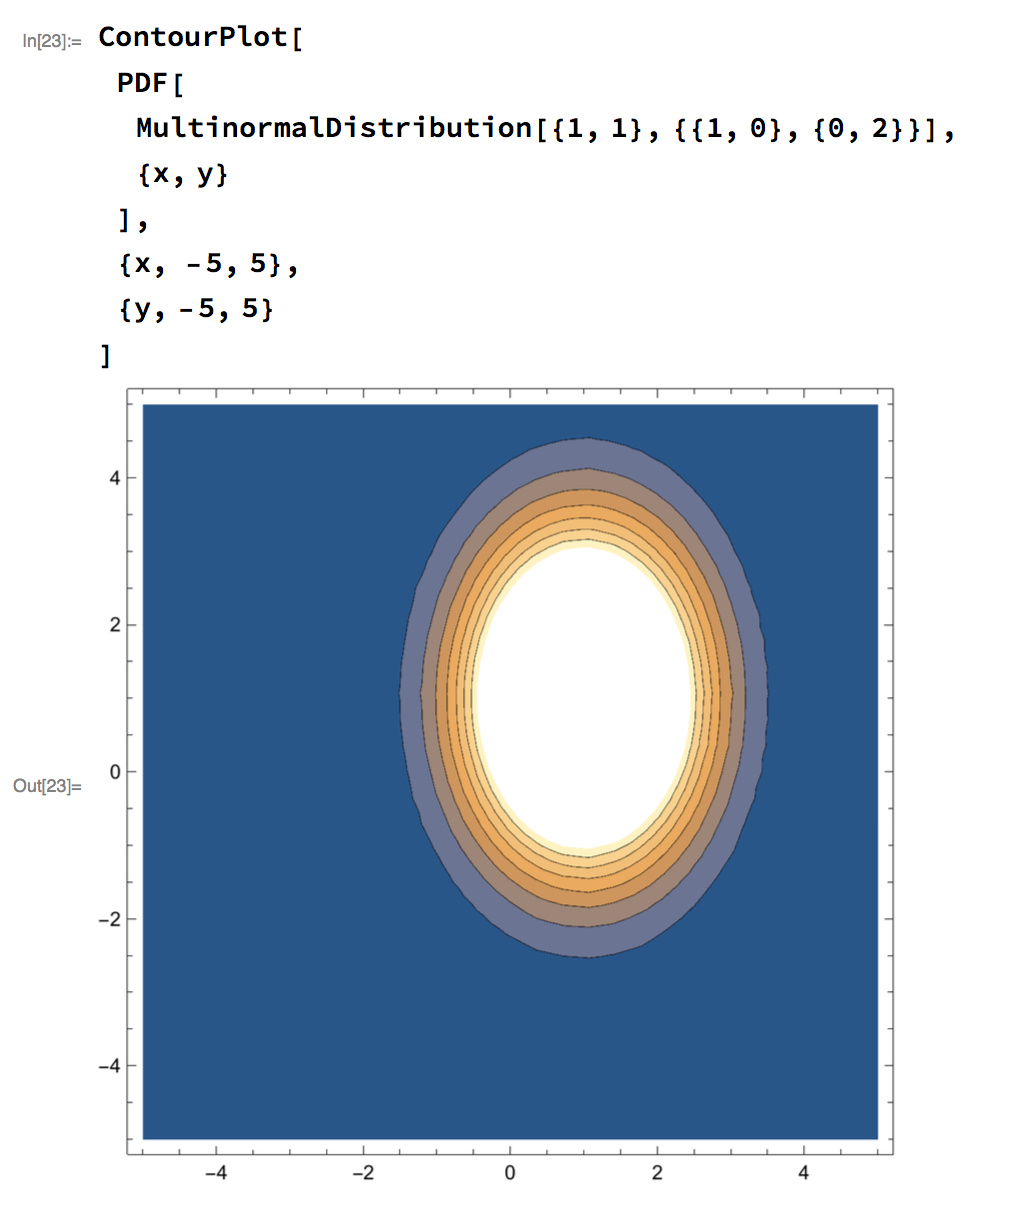
\includegraphics[width=300pt]{img/hw03_2a.png}
    \end{mdframed}
    \newpage
    \item $f(\mu, \Sigma)$, where $\mu = \begin{bmatrix}-1 \\ 2 \end{bmatrix}$ and $\Sigma = \begin{bmatrix} 2 & 1  \\ 1 & 3 \end{bmatrix}$.
    \begin{mdframed}
      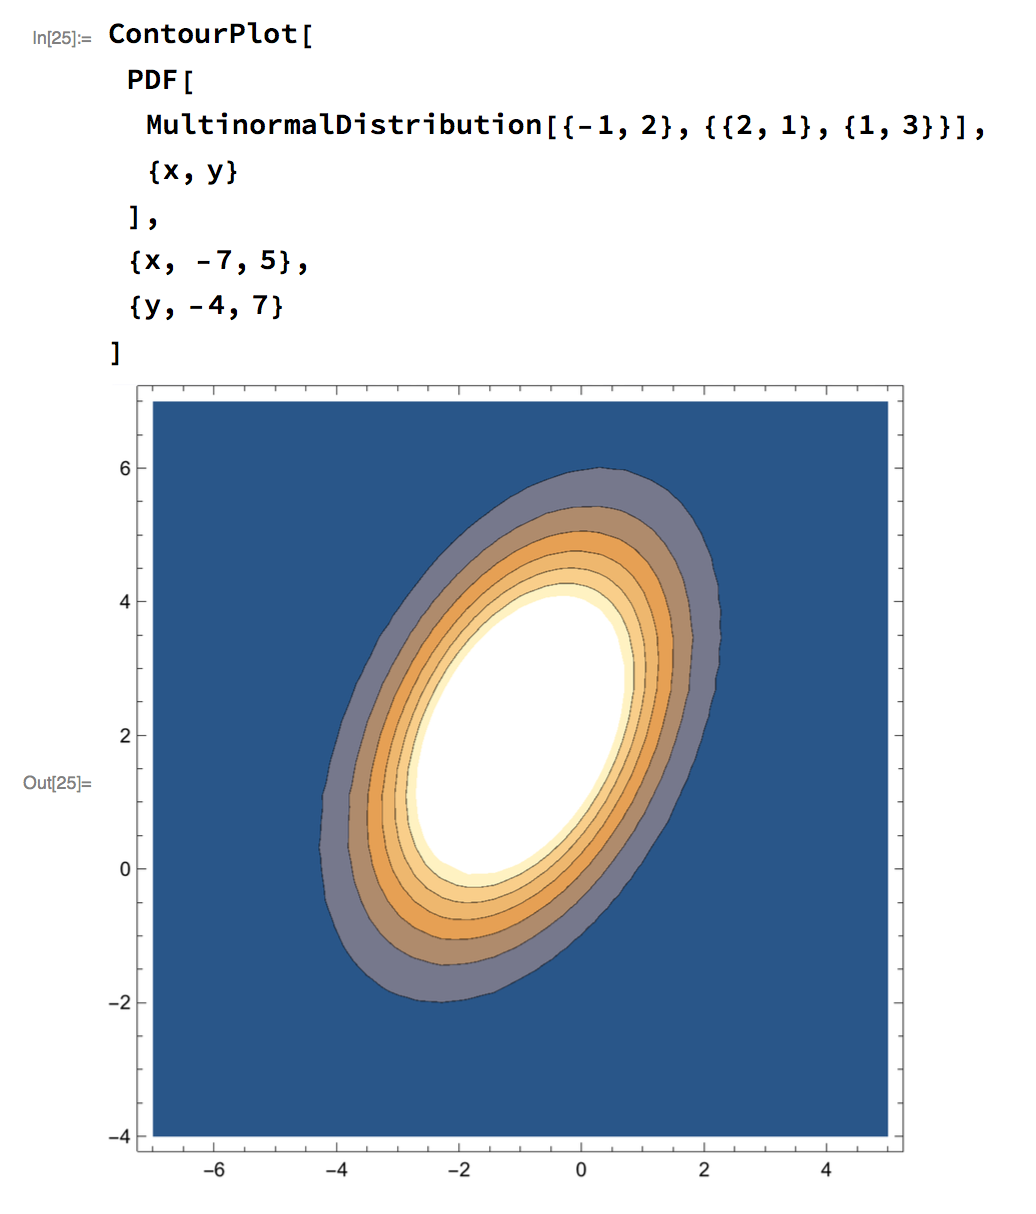
\includegraphics[width=300pt]{img/hw03_2b.png}
    \end{mdframed}

    \newpage
    \item $f(\mu_1, \Sigma_1) - f(\mu_2, \Sigma_2)$, where $\mu_1 = \begin{bmatrix} 0 \\ 2 \end{bmatrix}, \mu_2 = \begin{bmatrix} 2 \\ 0 \end{bmatrix}$ and $\Sigma_1 = \Sigma_2 = \begin{bmatrix} 2 & 1 \\ 1 & 1 \end{bmatrix}$.
    \begin{mdframed}
      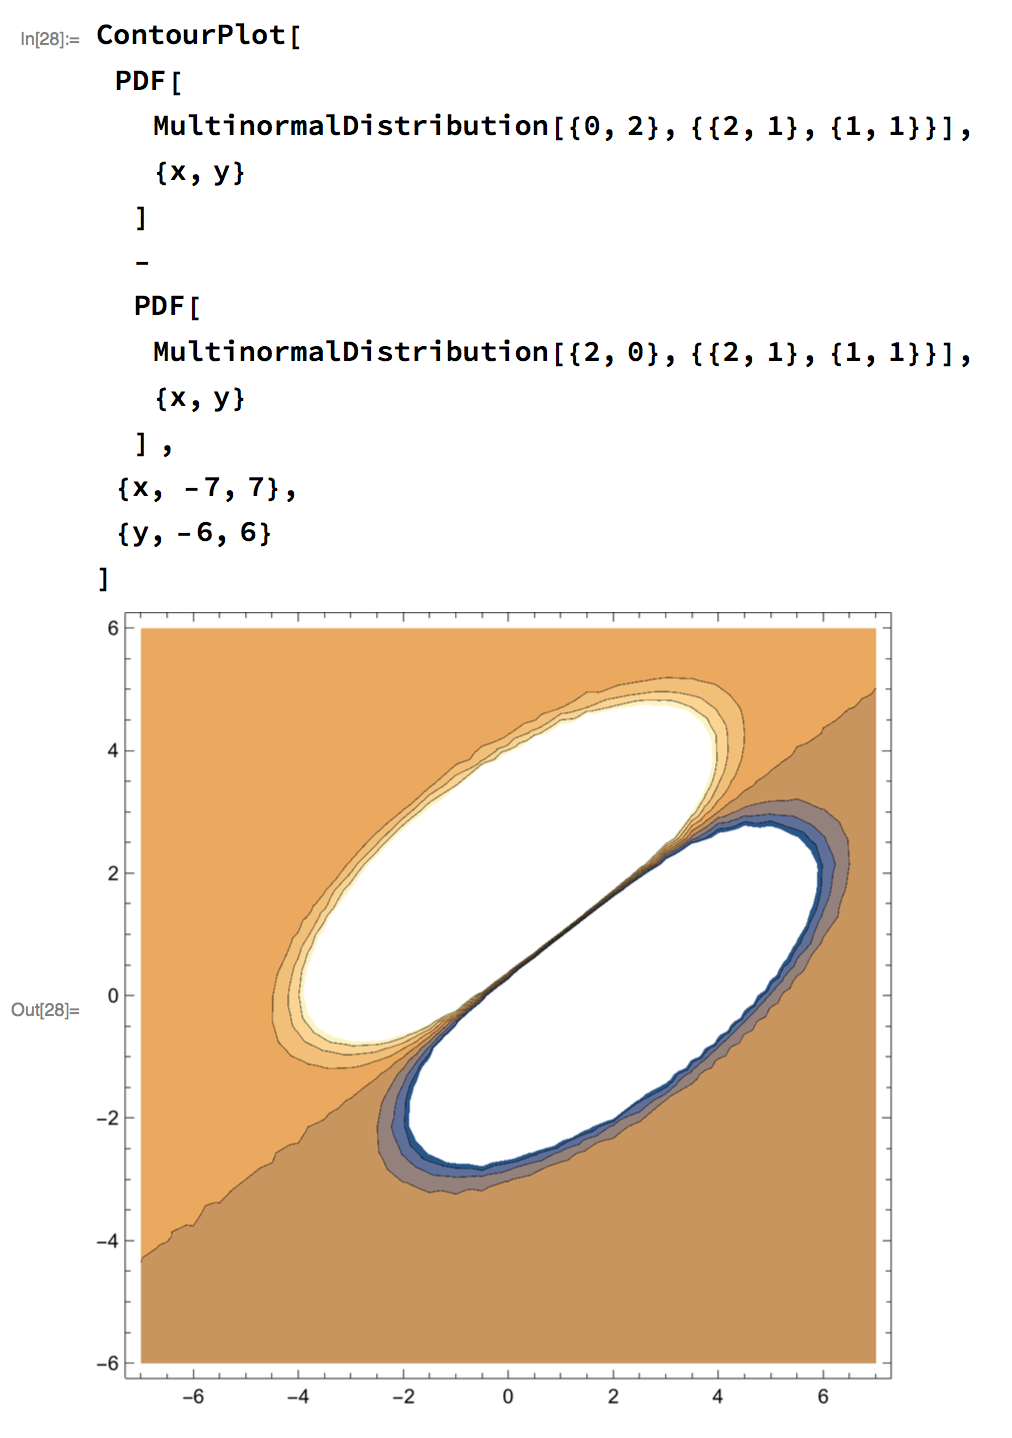
\includegraphics[width=300pt]{img/hw03_2c.png}
    \end{mdframed}

    \newpage
    \item $f(\mu_1, \Sigma_1) - f(\mu_2, \Sigma_2)$, where $\mu_1 = \begin{bmatrix} 0 \\ 2 \end{bmatrix}, \mu_2 = \begin{bmatrix} 2 \\ 0 \end{bmatrix}, \Sigma_1 = \begin{bmatrix} 2 & 1 \\ 1 & 1 \end{bmatrix}$ and $\Sigma_2 = \begin{bmatrix} 2 & 1 \\ 1 & 3 \end{bmatrix}$.
    \begin{mdframed}
      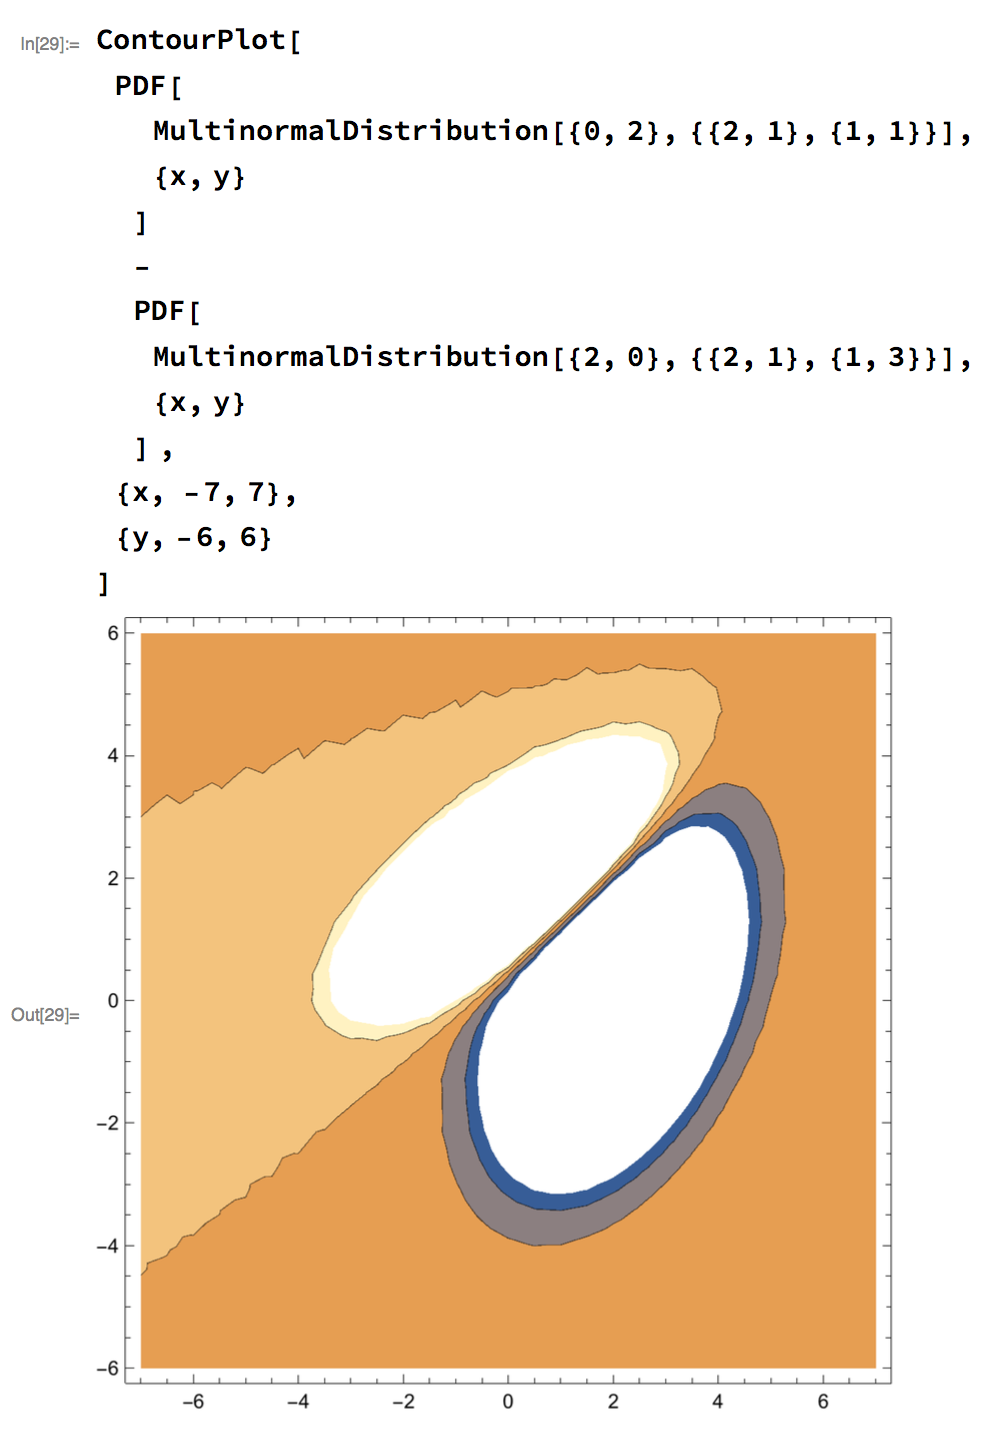
\includegraphics[width=300pt]{img/hw03_2d.png}
    \end{mdframed}

    \newpage
    \item $f(\mu_1, \Sigma_1) - f(\mu_2, \Sigma_2)$, where $\mu_1 = \begin{bmatrix} 1 \\ 1 \end{bmatrix}, \mu_2 = \begin{bmatrix} -1 \\ -1 \end{bmatrix}, \Sigma_1 = \begin{bmatrix} 2 & 0 \\ 0 & 1 \end{bmatrix}$ and $\Sigma_2 = \begin{bmatrix} 2 & 1 \\ 1 & 2 \end{bmatrix}$.
    \begin{mdframed}
      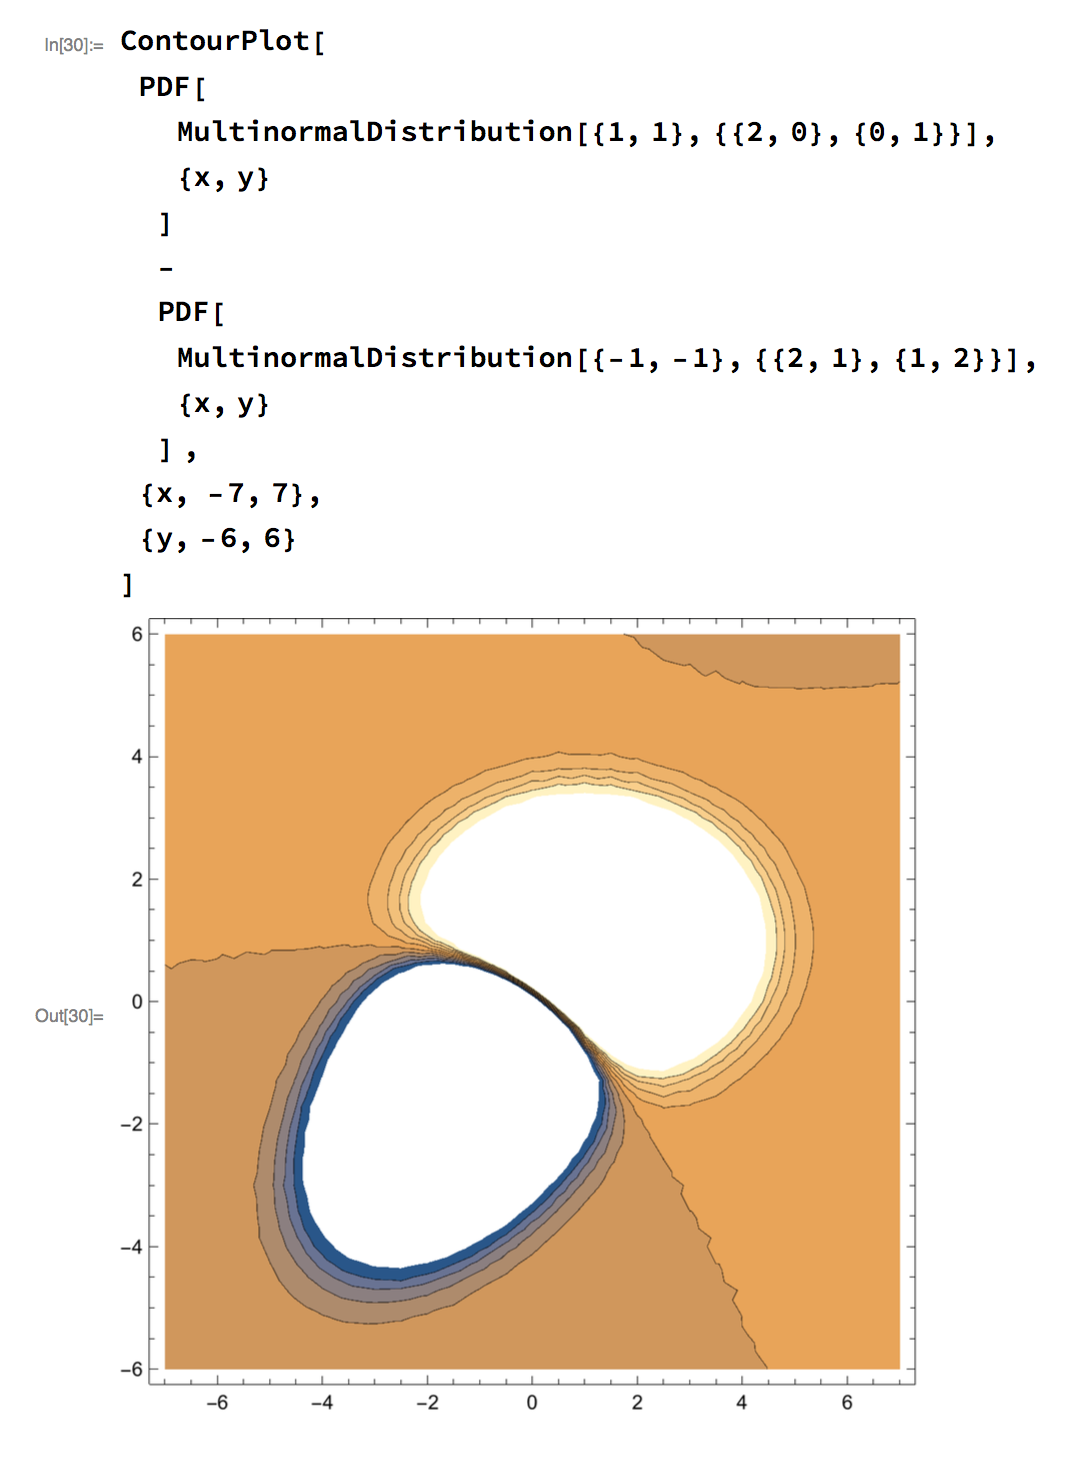
\includegraphics[width=300pt]{img/hw03_2e.png}
    \end{mdframed}

\end{enumerate}

\newpage
\subsection{Eigenvectors of the Gaussian Covariance Matrix}
Consider two one-dimensional random variables $X_1 \sim \N(3, 9)$ and $X_2 \sim \frac{1}{2}X_1 + \N(4, 4)$, where $\N(\mu, \sigma^2)$  is a Gaussian distribution with mean $\mu$ and variance $\sigma^2$. In software, draw $N = 100$ random two-dimensional sample points from $(X_1, X_2)$ such that the $i$th value sampled from $X_2$ is calculated based on the $i$th value sampled from $X_i$.
\begin{enumerate}[label=(\alph*)]
  \item
  \begin{mdframed}
    \begin{minted}{python}
      from numpy.random import normal

      X1 = normal(3, 3, 100)
      X2 = X1/2 + normal(4, 2, 100)
      X = np.stack([X1, X2], axis=1)
      n, d = X.shape
    \end{minted}
  \end{mdframed}
\item Compute the mean (in $\R^2$) of the sample.
  \begin{mdframed}
    \begin{minted}{python}
      mu = X.mean(axis=0)
    \end{minted}
  \end{mdframed}

\item Compute the $2 \times 2$ covariance matrix of the sample.
  \begin{mdframed}
    \begin{minted}{python}
      Sigma = (X - mu).T @ (X - mu) / (n * d)
    \end{minted}
  \end{mdframed}

\item Compute the eigenvectors and eigenvalues of this covariance matrix.
  \begin{mdframed}
    \begin{minted}{python}
      from numpy.linalg import eigh
      evals, evecs = eigh(Sigma)
    \end{minted}
  \end{mdframed}

\newpage
\item On a two-dimensional grid with a horizontal axis for $X_1$ with range $[-15, 15]$ and a vertical axis for $X_2$ with range $[-15, 15]$, plot
  \begin{enumerate}[label=(\roman*)]
  \item all $N=100$ data points, and
  \item arrows representing both covariance eigenvectors. The eigenvector arrows should originate at the mean and have magnitudes equal to their corresponding eigenvalues.
  \end{enumerate}
  \begin{mdframed}
    \begin{minted}{python}
      fig = plt.figure(figsize=(10,10))
      plt.xlim(-15,15)
      plt.ylim(-15,15)
      plt.scatter(X[:,0], X[:,1])
      arrow_kwargs = dict(fc="k", ec="k", head_width=0.3, head_length=0.5)
      plt.arrow(mu[0], mu[1],
      evecs[:,0][0] * evals[0],
      evecs[:,0][1] * evals[0],
      **arrow_kwargs)
      plt.arrow(mu[0], mu[1],
      evecs[:,1][0] * evals[1],
      evecs[:,1][1] * evals[1],
      **arrow_kwargs)
    \end{minted}
    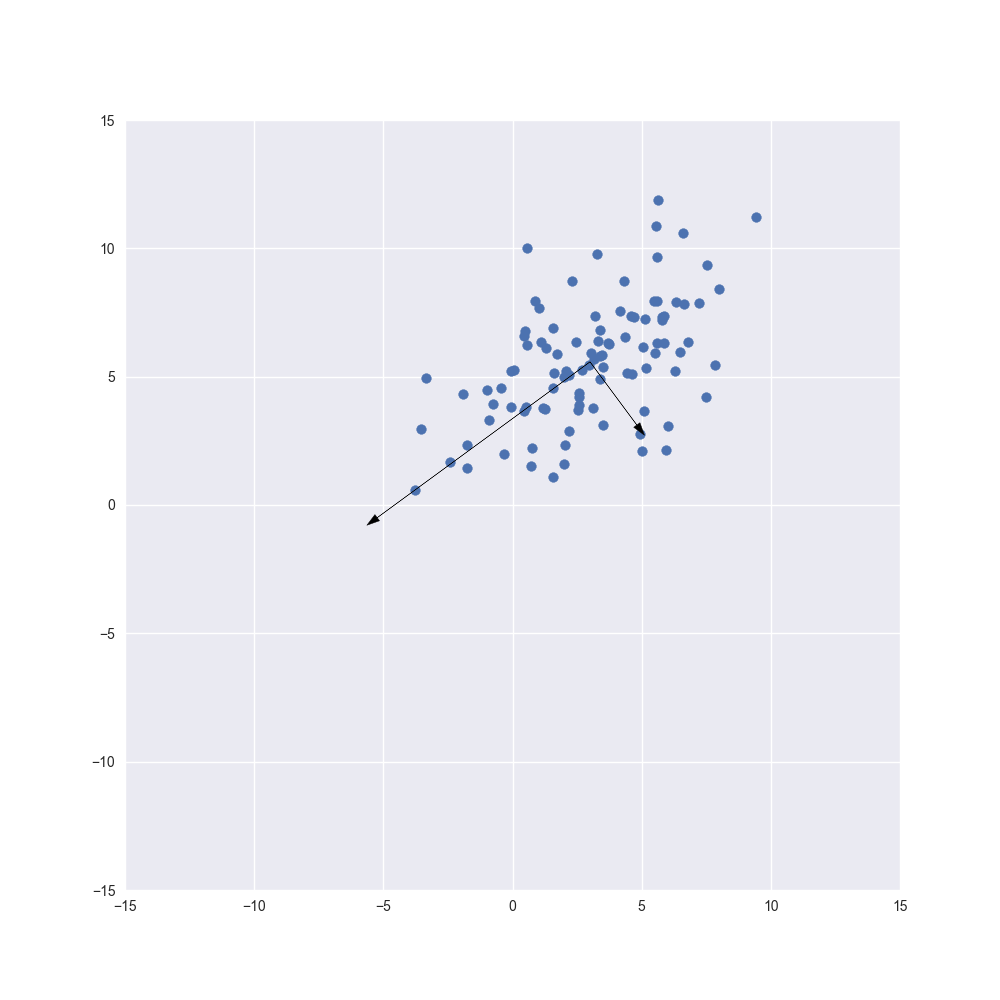
\includegraphics[width=300pt]{img/hw03_3d.png}
  \end{mdframed}

\newpage
\item Let $U = \begin{bmatrix} v_1 & v_2 \end{bmatrix}$ be a $2 \times 2$
  matrix whose columns are the eigenvectors of the covariance matrix, where
  $v_1$ is the eigenvector with the larger eigenvalue. We use $U^{\top}$ as a
  rotation matrix to rotate each sample point from the $(X_1, X_2)$ coordinate
  system to a coordinate system aligned with the eigenvectors. (As
  $U^{\top} = U^{-1}$, the matrix $U$ reverses this rotation, moving back from
  the eigenvector coordinate system to the original coordinate system). Center
  your sample points by subtracting the mean $\mu$ from each point; then rotate
  each point by $U^{\top}$, giving $x_{\text{rotated}} = U^{\top}(x - \mu)$.
  Plot these rotated points on a new two dimensional-grid, again with both axes
  having range $[-15, 15]$.
  \begin{mdframed}
    \begin{minted}{python}
      U = evecs[:,::-1]
      X_centered = X - mu
      X_centered_rotated = (U.T @ X_centered.T).T

      fig = plt.figure(figsize=(10,10))
      plt.xlim(-15,15)
      plt.ylim(-15,15)
      plt.scatter(X_centered_rotated[:,0], X_centered_rotated[:,1])
    \end{minted}
    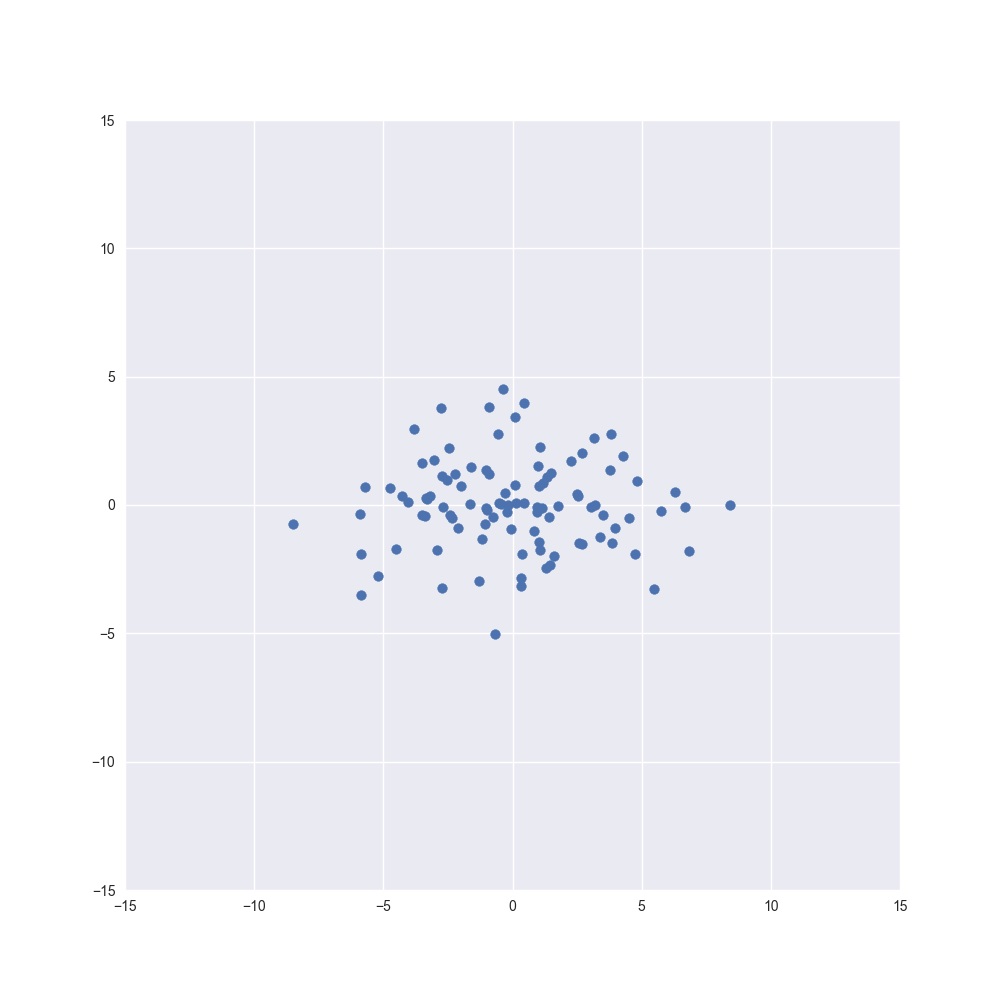
\includegraphics[width=300pt]{img/hw03_3e.png}
  \end{mdframed}

\end{enumerate}

\newpage
\subsection{Maximum Likelihood Estimation}
Let $X_1, \ldots, X_n \in \R^d$ be $n$ sample points drawn independently from a multivariate normal distribution $\N(\mu, \Sigma)$.
\begin{enumerate}[label=(\alph*)]
    \item Suppose the normal distribution has an unknown diagonal covariance matrix
    $$
    \Sigma =
    \begin{bmatrix}
    \sigma_1^2 & & & & \\
    & \sigma_2^2 & & & \\
    & & \sigma_3^2 & & \\
    & & & \ddots & \\
    & & & & \sigma_d^2 \\
    \end{bmatrix}
    $$
    and an unknown mean $\mu$. Derive the maximum likelihood estimates, denoted
    $\hat{\mu}$ and $\hat{\sigma_i}$ for $\mu$ and $\sigma_i$. Show all your
    work.

    (Answer starts on next page)

    \begin{mdframed}
      First, let's get some intuition for the situation: the covariance matrix
      is diagonal, so the isocontours of the PDF of the Gaussian are
      axis-aligned. That means that the PDF can be factored into a product of
      one-dimensional marginal densities: i.e. we can compute the density of a
      sample vector $\vec x$ as the product of densities of its scalar
      components (individual features):
      $\p(\vec x;\vec \mu, \vec \Sigma) = \prod_{j=1}^d \p(\vec x_j; \mu_j,
      \sigma^2_j)$. We therefore expect the estimation problem to be fairly
      straightforward, essentially involving fitting $d$ one-dimensional
      Gaussians independently.

      The likelihood function is
      \begin{align*}
        \L(\mu, \Sigma)
        &= \prod_{i=1}^n \p(X_i;\mu, \Sigma) \\
        &= \prod_{i=1}^n \prod_{j=1}^d \p(\vec X_{ij}; \mu_j, \sigma^2_j) \\
        &= \prod_{i=1}^n \prod_{j=1}^d \frac{1}{(\sqrt{2\pi})^d \sigma_j^d} \exp\(\frac{-(X_{ij} - \mu_j)^2}{2\sigma_j^2}\), \\
      \end{align*}
      giving the log-likelihood function
      \begin{align*}
        \l(\mu, \Sigma)
        &= \sum_{i=1}^n \sum_{j=1}^d -d\log\sigma_j - \frac{(X_{ij} - \mu_j)^2}{2\sigma_j^2} + \constant \\
        &= \sum_{j=1}^d -nd\log\sigma_j - \frac{1}{2\sigma_j^2} \sum_{i=1}^n  (X_{ij} - \mu_j)^2  + \constant. \\
      \end{align*}
      Fix a particular feature $j$. The partial derivatives with respect to the
      mean and variance parameter for that feature are
      \begin{align*}
        \dldmuj &= \frac{1}{\sigma^2_j}\sum_{i=1}^n(X_{ij} - \mu_j) = \frac{1}{\sigma^2_j}\(-n\mu_j + \sum_{i=1}^nX_{ij}\)\\
        \dldsigmaj &= -\frac{nd}{\sigma_j} + \frac{1}{\sigma_j^3} \sum_{i=1}^n  (X_{ij} - \mu_j)^2.
      \end{align*}
      To find the MLE $\hat \mu_j$ we set the partial derivative equal to zero
      and solve for $\mu$:
      \begin{align*}
        \dldmuj = 0
        &\implies -n\hat \mu_j + \sum_{i=1}^nX_{ij} = 0\\
        &\implies \hat \mu_j = \frac{1}{n}\sum_{i=1}^nX_{ij}.
      \end{align*}
      To find the MLE $\hat \sigma_j$ we set the partial derivative equal to
      zero, set $\mu_j = \hat \mu_j$, and solve for $\sigma$:
      \begin{align*}
        \dldsigmaj = 0
        &\implies -nd + \frac{1}{\hat \sigma_j^2} \sum_{i=1}^n  (X_{ij} - \hat \mu_j)^2 = 0 \\
        &\implies \hat \sigma_j^2 = \frac{1}{nd}\sum_{i=1}^n  (X_{ij} - \hat \mu_j)^2.
      \end{align*}
      (Why is it valid to substitute $\hat \mu_j$ for $\mu_j$?)
    \end{mdframed}

    \begin{mdframed}
      To verify that these critical points are indeed maxima, we note first
      that $\l(\mu, \Sigma)$ is a quadratic in $\mu$, in which the sign of
      $\mu_j$ is negative. Therefore it is a concave-down quadratic in $\mu_j$
      and has only a maximum; no minimum.

      For $\sigma$ we compute the second partial derivative,
      \begin{align*}
        \ddldsigmajsigmaj = \frac{nd}{\sigma_j^2} - \frac{3}{\sigma_j^4} \SS_j,
      \end{align*}
      where $\SS_j = \sum_{i=1}^n  (X_{ij} - \mu_j)^2$, and evaluate it at the critical point:
      \begin{align*}
        \ddldsigmajsigmaj(\sigma_j)
        &= \frac{(nd)^2}{\SS_j} - \frac{3(nd)^4}{\(\SS_j\)^4} \SS_j\\
        &= \frac{(nd)^2}{\SS_j} - \frac{3(nd)^4}{\(\SS_j\)^3}.\\
      \end{align*}
      (I was expecting to be able to show that $\ddldsigmajsigmaj(\sigma_j)$ is
      negative but I don't seem to be managing to do so.)
    \end{mdframed}

    \newpage
  \item Suppose the normal distribution has a known covariance matrix $\Sigma$
    and an unknown mean $A \mu$, where $\Sigma$ and $A$ are known $d \times d$
    matrices, $\Sigma$ is positive definite, and $A$ is invertible.  Derive the
    maximum likelihood estimate, denoted $\hat{\mu}$, for $\mu$.
    \begin{mdframed}
      % Let's change coordinate system so that the mean of the Gaussian is
      % $\mu$. Clearly we can do this by applying the transformation $A^\1$.  In
      % this coordinate system, the sample points are the rows of
      % $X' = (A^\1X^\T)^\T$ ($A$ is a covariance matrix of a Gaussian, hence
      % symmetric positive definite, hence invertible).

      % The mean of the rows of $X'$ is $A^\1A\mu = \mu$.

      Let $\eta = A\mu$. Then $\hat \eta_j = \frac{1}{n}\sum_{i=1}^nX_{ij}$ as
      above. There is a theorem (the ``invariance property'') regarding MLEs
      which states that $\hat{g(\theta)}$ is $g(\hat \theta)$, where $\hat~$
      denotes MLE.

      We know $\hat{A\mu}$. We want $\hat{\mu} = \hat{A^\1A\mu}$. By the
      invariance property for MLEs this is
      $$
      \hat \mu = A^\1\hat{A\mu} = A^\1\frac{1}{n}\sum_{i=1}^nX_{ij}.
      $$
      I'm not entirely sure what requirements this theorem makes of $g$ but I
      am confident that the invertible linear transformation $A^\1$ satisfies
      them.

      Alternatively, without relying on this theorem, I tried to argue from
      first principles, but currently am confused when attempting to compute the
      gradient for $\mu$:

      The likelihood function for $\mu$ is
      \begin{align*}
        \L(\mu)
        &= \prod_{i=1}^n \frac{1}{\(\sqrt{2\pi}\)^d\sqrt{|\Sigma|}}\exp\(-\frac{1}{2}(X_i - A\mu)^\T\Sigma^\1(X_i - A\mu)\),
      \end{align*}
      and the log-likelihood function is
      \begin{align*}
        \l(\mu)
        &= -\frac{1}{2}\sum_{i=1}^n (X_i - A\mu)^\T\Sigma^\1(X_i - A\mu) + \constant.
      \end{align*}
      % The first derivative with respect to $\mu$ is
      % \begin{align*}
      %   \dldmu = \sum_{i=1}^n (X_i - A\mu)^\T\Sigma^\1A
      % \end{align*}

      Let $\dot X_i = X_i - A\mu$. Then the log-likelihood is the following
      quadratic form (up to an additive constant):
      \begin{align*}
        \l(\mu)
        &= -\frac{1}{2}\sum_{i=1}^n \dot X_i^\T\Sigma^\1 \dot X_i\\
        &= -\frac{1}{2}\sum_{i=1}^n\sum_{j=1}^d\sum_{k=1}^d \(\Sigma^\1\)_{jk} \dot X_{ij} \dot X_{ik}\\
        &= -\frac{1}{2}\sum_{i=1}^n\sum_{j=1}^d\sum_{k=1}^d \(\Sigma^\1\)_{jk} \(X_{ij} - (A\mu)_j\) \(X_{ik} - (A\mu)_k\)\\
        &= -\frac{1}{2}\sum_{j=1}^d\sum_{k=1}^d \(\Sigma^\1\)_{jk} \sum_{i=1}^n (X_{ij} - (A\mu)_j) (X_{ik} - (A\mu)_k)\\
        &= -\frac{1}{2}\sum_{j=1}^d\sum_{k=1}^d \(\Sigma^\1\)_{jk} \sum_{i=1}^n \(X_{ij}X_{ik} - X_{ik}(A\mu)_j - X_{ij}(A\mu)_k + (A\mu)_j(A\mu)_k\)\\
      \end{align*}



    \end{mdframed}

\end{enumerate}

\newpage
\subsection{Covariance Matrices and Decompositions}
As described in lecture, the covariance matrix $\text{Var}(R) \in \R^{d\times d}$ for a random variable $R \in \R^d$ with mean $\mu$ is
$$
\text{Var}(R) = \text{Cov}(R, R) = \E[(R- \mu)(R-\mu)^{\top}] =
\begin{bmatrix}
\Var(R_1) & \Cov(R_1, R_2) & \ldots & \Cov(R_1, R_d) \\
\Cov(R_2, R_1) & \Var(R_2) & & \Cov(R_2, R_d) \\
\vdots & & \ddots & \vdots \\
\Cov(R_d, R_1) & \Cov(R_d, R_2) & \ldots & \Var(R_d)
\end{bmatrix}
$$
where $\Cov(R_i, R_j) = \E[(R_i - \mu_i)(R_j - \mu_j)]$ and $\Var(R_i) = \Cov(R_i, R_i)$. \\

\noindent
If the random variable $R$ is sampled from the multivariate normal distribution $\N(\mu, \Sigma)$ with the PDF
$$ f(x) = \frac{1}{\sqrt{(2\pi)^d |\Sigma|}} e^{((x-\mu)^{\top}\Sigma^{-1}(x-\mu))/2},$$
then $\Var(R) = \Sigma$.\\

\noindent
Given $n$ points $X_1, X_2, \ldots, X_n$ sampled from $\N(\mu, \Sigma)$, we can estimate $\Sigma$ with the maximum likelihood estimator
$$ \hat{\Sigma} = \frac{1}{n} \sum_{i=1}^n (X_i - \mu)(X_i - \mu)^{\top},$$ which is also known as the covariance matrix of the sample
\begin{enumerate}[label=(\alph*)]
\item The estimate $\hat{\Sigma}$ makes sense as an approximation of $\Sigma$
  only if $\hat{\Sigma}$ is invertible. Under what circumstances is
  $\hat{\Sigma}$ not invertible? Make sure your answer is complete; i.e., it
  includes all cases in which the covariance matrix of the sample is
  singular. Express you answer in terms of the geometric arrangement of the
  sample points Xi.
    \begin{mdframed}
      Let $\dot X$ represent the centered data, i.e. $\dot X_i = X_i - \mu$.

      Note that $\hat \Sigma$ is the mean of a collection of $n$ outer product
      matrices $\dot X_i \dot X_i^\T$, where each outer product matrix is
      contributed by a single sample point. Also note that the columns of
      $\dot X_i \dot X_i^\T$ are all scalar multiples of $\dot X_i$.

      $\hat \Sigma$ is invertible if and only if it is full-rank. Full-rank
      means that its columns are linearly independent.

      From this point of view, the following circumstances will lead to
      $\hat \Sigma$ being singular:

      \begin{enumerate}
      \item \textbf{There is only one point.} If $n = 1$ then $\mu = X_1$ and
        $\dot X_1 = \vec 0$, and the outer product is the zero matrix. This is
        singular (e.g. determinant is zero).
      \item \textbf{$d > 1$ and there are only two points.} If $n = 2$ then
        $\mu$ lies on the line connecting the two points, so
        $\dot X_1 = a\dot X_2$ for some scalar $a$. Therefore the columns of
        the sum of the two outer product matrices differ only by a scalar
        multiple.
      \end{enumerate}

      In general, the centered sample vectors $\{\dot X_i: 1 < i \leq n\}$ must
      span $\R^d$. I.e. if the sample vectors lie in an affine hyperplane of
      $\R^d$ then $\hat \Sigma$ will be singular.

    \end{mdframed}

  \item Suggest a way to fix a singular covariance matrix estimator
    $\hat{\Sigma}$ by replacing it with a similar but invertible matrix. Your
    suggestion may be a kludge, but it should not change the covariance matrix
    too much. Note that infinitesimal numbers do not exist; if your solution
    uses a very small number, explain how to calculate a number that is
    sufficiently small for your purposes.
    \begin{mdframed}
      In my code I have used the pseudoinverse function
      \texttt{numpy.linalg.pinv}.
    \end{mdframed}

  \item Consider the normal distribution $\N(0, \Sigma)$ with mean $\mu =
    0$. Consider all vectors of length 1; i.e., any vector $x$ for which
    $|x| =1$. Which vector(s) $x$ of length 1 maximizes the PDF $f(x)$? Which
    vector(s) $x$ of length 1 minimizes $f(x)$? (Your answers should depend on
    the properties of $\Sigma$.) Explain your answer.
    \begin{mdframed}
      Let $\vec v_1, \vec v_2, \ldots, \vec v_n$ be unit-length eigenvectors of
      $\Sigma$, arranged in order of decreasing eigenvalue.

      Note that $f(x)$ is maximum at the mean $\vec 0$ and decreases with
      increasing distance from $\vec 0$. The exact form of this decrease is
      determined by the quadratic form
      $(\vec x - \mu)^\T\Sigma^\1 (\vec x - \mu)$.

      Then the unit vector $x$ that maximizes $f(\vec x)$ is $\vec v_n$. This
      is because the eigenvector with smallest eigenvalue points in the
      direction of least slope of the quadratic form. Similarly, $\vec v_1$ is
      the unit vector that minimizes $f(\vec x)$ because the eigenvector with
      largest eigenvalue points in the direction of greatest slope of the
      quadratic form.
    \end{mdframed}
\end{enumerate}

\newpage
\subsection{Gaussian Classifiers for Digits and Spam}
In this problem, you will build classifiers based on Gaussian discriminant analysis. Unlike Homework 1, you are NOT allowed to use any libraries for out-of-the-box classification (e.g \texttt{sklearn}). You may use anything in \texttt{numpy} and \texttt{scipy}. \\

\noindent
The training and test data can be found on Piazza in the post corresponding to this homework. Don’t use the training/test data from Homework 1, as they have changed for this homework. Submit your predicted class labels for the test data on the Kaggle competition website and be sure to include your Kaggle display name and scores in your writeup. Also be sure to include an appendix of your code at the end of your writeup.

\begin{enumerate}[label=(\alph*)]
\item Taking pixel values as features (no new features yet, please), fit a
  Gaussian distribution to each digit class using maximum likelihood
  estimation. This involves computing a mean and a covariance matrix for each
  digit class, as discussed in lecture. \emph{Tip}: You may, and probably
  should, contrast-normalize the images before using their pixel values. One
  way to normalize is to divide the pixel values of an image by the $l_2$ norm
  of its pixel values.
\item (Written answer) Visualize the covariance matrix for a particular class
  (digit). How do the diagonal terms compare with the off-diagonal terms? What
  do you conclude from this?
    \begin{mdframed}
      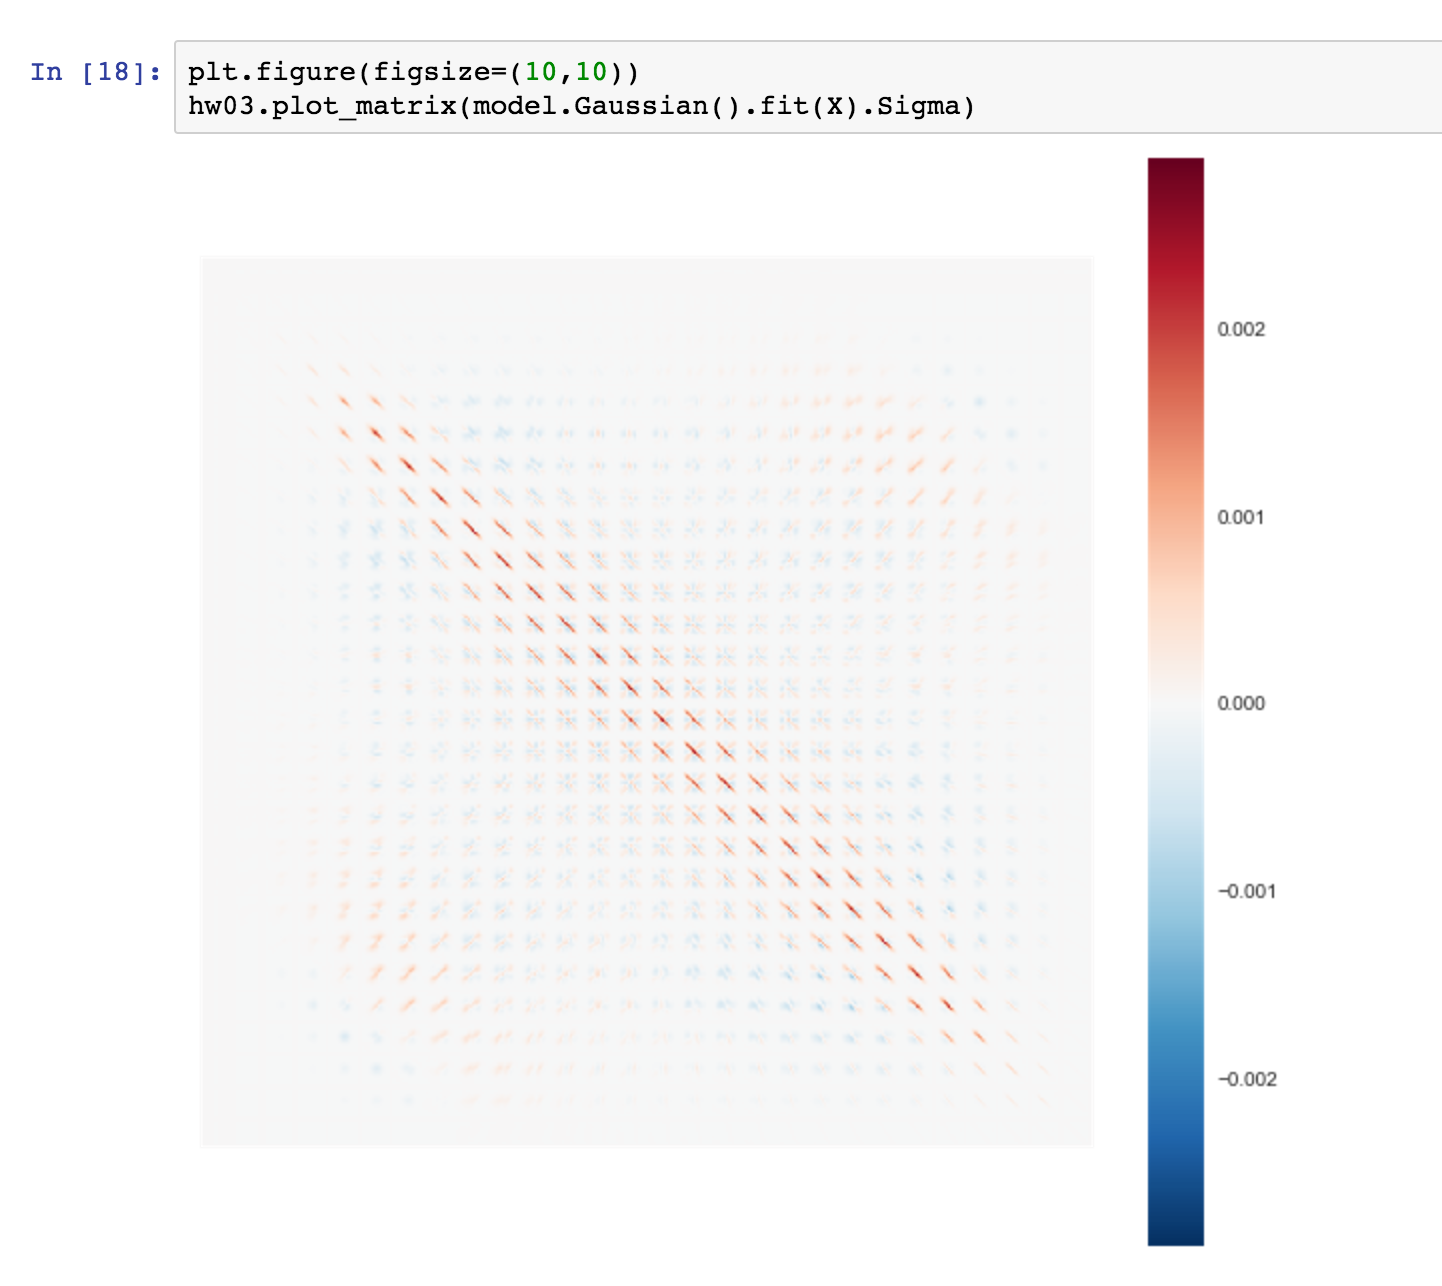
\includegraphics[width=300pt]{img/hw03_6b.png}
    \end{mdframed}

  \item Classify the digits in the test set on the basis of posterior
    probabilities with two different approaches.
    \begin{enumerate}[label=(\roman*)]
        \item Linear discriminant analysis (LDA). Model the class conditional probabilities as Gaussians $\N(\mu_C, \Sigma)$ with different means $\mu_C$ (for class C) and the same covariance matrix $\Sigma$, the average covariance matrix of the 10 classes. \\

        Hold out 10,000 randomly chosen training points for a validation set. Classify each image in the validation set into one of the 10 classes (with a 0-1 loss function). Compute the error rate and plot it over the following numbers of randomly chosen training points: $$[100, 200, 500, 1,000, 2,000, 5,000, 10,000, 30,000, 50,000].$$ (Expect some variance in your error rate when few training points are used.)

        \item Quadratic discriminant analysis (QDA). Model the class conditionals as Gaussians $\N(\mu_C, \Sigma_C)$, where $\Sigma_C$ is the estimated covariance matrix for class C. (If any of these covariance matrices turn out singular, implement the trick you described in Q5.(b). You are welcome to use $k$-fold cross validation to choose the right constant(s) for that trick.) Repeat the same tests and error rate calculations you did for LDA.

        \item  (Written answer.) Which of LDA and QDA performed better? Why?
        \begin{mdframed}
          My QDA implementation is currently incorrect. The unit tests pass for
          1 and 2D cases but when the sample points are higher-dimensional QDA
          is classifying points essentially uniformly at random (around 90\%
          error rate).
          \\\\
          Here are the error rates for my LDA implementation using the provided
          data, with contrast normalization.
          \\\\
          \begin{tabular}{l|l}
            \#{training points}&Error rate\\
            \hline
            100 & 0.51\\
            200 & 0.91\\
            500 & 0.78\\
            1000 & 0.36\\
            2000 & 0.34\\
            5000 & 0.31\\
            10000 & 0.34\\
            30000 & 0.29\\
            50000 & 0.28\\
          \end{tabular}
        \end{mdframed}

      \item Train your best classifier with \texttt{train.mat} and classify the
        images in \texttt{test.mat}. Submit your labels to the online Kaggle
        competition. Record your optimum prediction rate in your
        submission. You are welcome to compute extra features for the Kaggle
        competition. If you do so, please describe your implementation in your
        assignment. Please use extra features \textbf{only} for this portion of
        the assignment. In your submission, include plots of error rate versus
        number of training examples for both LDA and QDA. Also include tables
        giving the error rates (as percentages) for each number of training
        examples for both LDA and QDA. Include written answers where indicated.
        \begin{mdframed}
          0.77 accuracy score for digits; LDA.
        \end{mdframed}

    \end{enumerate}
  \item Next, apply LDA or QDA (your choice) to spam. Submit your test results to the online Kaggle competition. Record your optimum prediction rate in your submission. If you use additional features (or omit features), please describe them. \\

      \emph{Optional:} If you use the defaults, expect relatively low
      classification rates. The TAs suggest using a bag-of-words model. You may
      use third-party packages to implement that if you wish. Also, normalizing
      your vectors might help.

    \begin{mdframed}
      0.71 accuracy score for spam; LDA.
    \end{mdframed}

    \item \emph{Extra for Experts:} Using the \texttt{training\_data} and \texttt{training\_labels} in \texttt{spam.mat}, identify 10 words in your features set corresponding to the maximum and minimum variances. Use $k$-fold cross validation to train your classifier using only 10 variance-maximum words and record your average error rate. Do the same with the 10 minimum-variance words. What do you notice?
    \begin{mdframed} \solution
    % SOLUTION HERE
    \end{mdframed}
\end{enumerate}


\newcommand{\bb}{{\mathbf{b}}}
\newcommand{\bx}{{\mathbf{x}}}
\newcommand{\bmu}{{\mathbf{\mu}}}
\newcommand{\bX}{{\mathbf{X}}}
%\newcommand{\by}{{\mathbf{y}}}
\newcommand{\bY}{{\mathbf{Y}}}
\newcommand{\bz}{{\mathbf{z}}}
\newcommand{\bw}{{\mathbf{w}}}

\newcommand{\auth}[1]{}
\newcommand{\com}[1]{(#1)}
\newcommand{\delete}[1]{}

\newcommand{\todo}[1]{\textcolor{blue}{#1}}
\def\P{{\mathbb P}}
\def\E{{\mathbb E}}
\def\1{{\mathbf 1}}

\section{Homework 4 - Regression}

\subsection{Logistic Regression with Newton's Method}

Consider sample points $X_1, X_2, \ldots, X_n \in \mathbb{R}^d$ and
associated values $y_1, y_2, \ldots, y_n \in \{ 0, 1 \}$,
an $n \times d$ design matrix $X = [X_1~~~~\dots~~~~X_n]^{\T}$ and
an $n$-vector $y = [y_1~~~~\dots~~~~y_n]^{\T}$.

If we add $\ell_2$-regularization to logistic regression,
the cost function is
\[
J(w) = \lambda \, |w|^2_2 -
\sum_{i=1}^n \left(y_i \ln s_i + (1-y_i) \ln (1 - s_i) \rule{0pt}{18pt} \right)
\]
where $s_i = s(X_i \cdot w)$, $s(\gamma) = 1 / (1 + e^{- \gamma})$, and
$\lambda > 0$ is the regularization parameter.
As in lecture, the vector $s = [s_1~~~~\dots~~~~s_n]^{\T}$ is
a useful shorthand.

In this problem, you will use Newton's method to minimize this cost function
on the four-point, two dimensional training set
\[
X = \begin{bmatrix} 0 &3 \\ 1& 3\\ 0 &1\\ 1 &1 \end{bmatrix},
\hspace{1in}
y = \begin{bmatrix} 1\\1\\0\\0 \end{bmatrix}.
\]
You may want to draw these points on paper to see what they look like.
The $y$-vector implies that the first two sample points are in class $1$, and
the last two are in class $0$.

These sample points cannot be separated by a decision boundary that
passes through the origin.
As described in lecture, append a $1$ to each $X_i$ vector and
use a weight vector $w \in \mathbb{R}^3$ whose last component is
the bias term (the term we call $\alpha$ in lecture).

\begin{enumerate}
\item
Derive the gradient of the cost function $J(w)$.
Your answer should be a simple matrix-vector expression.
Do NOT write your answer in terms of the individual components of
the gradient vector.

\begin{comment}
\begin{mdframed}
\textbf{Initial verbose version}:

The gradient of the cost function is
\begin{align*}
  \nabla J(\w) = \lambda \nabla |\w|^2 - \sum_i
  y_i     \nabla \ln s_i(\w) +
  (1-y_i) \nabla \ln(1 - s_i(\w)).
\end{align*}
Let's compute the three derivatives separately.
\hlinee
First the regularization term:
\begin{align*}
  \nabla |\w|^2 = \nabla \sum_{j=1}^d w_j^2 = \cvecccc{2w_1}{\vdots}{2w_d}{2\alpha} = 2\w.
\end{align*}
\hlinee
Next $\ln s_i(\w)$. The partial derivative with respect to one component $w_j$ is
\begin{align*}
  \partiald{\ln s_i(\w)}{w_j}
  = \frac{1}{s_i(\w)} \partiald{s_i(\w)}{w_j}
\end{align*}
and the partial derivative of the logistic function is
\begin{align*}
  \partiald{s_i(\w)}{w_j} &= \partiald{~(1 + e^{-\w \cdot \x_i})^{-1}}{w_j} \\
  &= -(1 + e^{-\w \cdot \x_i})^{-2} (-x_{ij})e^{-\w\cdot\x_i} \\
  &= x_{ij}\frac{e^{-\w\cdot\x_i}}{(1 + e^{-\w \cdot \x_i})^2} \\
  &= x_{ij}s_i(\w)(1 - s_i(\w)),
\end{align*}
so putting the last two results together gives
\begin{align*}
  \partiald{\ln s_i(\w)}{w_j} = x_{ij}(1 - s_i(\w)),
\end{align*}
and therefore the gradient of $\ln s_i(\w)$ is
\begin{align*}
  \nabla \ln s_i(\w) =
\cvecccc
{\partiald{\ln s_i(\w)}{w_1}}
{\vdots}
{\partiald{\ln s_i(\w)}{w_d}}
{\partiald{\ln s_i(\w)}{\alpha}}
=
\cvecccc
{x_{i1}(1 - s_i(\w))}
{\vdots}
{x_{id}(1 - s_i(\w))}
{1 - s_i(\w)}
= (1 - s_i(\w))\x_i.
\end{align*}
\hlinee
Now $\ln(1 - s_i(\w))$. We've already computed $(s_i(\w))'$, so
\begin{align*}
  \partiald{\ln \(1 - s_i(\w)\)}{w_1}
  &= \frac{1}{1 - s_i(\w)}(-1)x_{ij}s_i(\w)(1 - s_i(\w)) \\
  &= -x_{ij}s_i(\w),
\end{align*}
and
\begin{align*}
  \nabla \ln (1 - s_i(\w)) =
\cvecccc
{-x_{i1}s_i(\w)}
{\vdots}
{-x_{id}s_i(\w)}
{-s_i(\w)} =
-s_i(\w)\x_i.
\end{align*}
\hlinee
Finally, putting the three derivatives together gives the gradient of the cost function:
\begin{align*}
  \nabla J(\w)
  &= \lambda \nabla |\w|^2 - \sum_i
  y_i     \nabla \ln s_i(\w) +
  (1-y_i) \nabla \ln(1 - s_i(\w)) \\
  &= 2\lambda\w - \sum_i y_i (1 - s_i(\w))\x_i - (1 - y_i) s_i(\w)\x_i \\
  &= 2\lambda\w - \sum_i y_i\x_i - s_i(\w)\x_i \\
  &= 2\lambda\w - \X^\T\y - \X^\T s(\X\w) \\
  &= 2\lambda\w - \X^\T(\y - s(\X\w)),
\end{align*}
where
$s(\X\w) = \cveccc{1/(1+e^{-\X_1\cdot\w})}{\vdots}{1/(1+e^{-\X_n\cdot\w})}$
contains the predicted values (class probability) for each sample point, given
parameters $\w$.
\end{mdframed}
\end{comment}

\begin{comment}
\begin{mdframed}
\textbf{Second version, not using chain rule}:
First note that
\begin{align*}
  \partiald{s_i(\w)}{w_j} &= \partiald{~(1 + e^{-\w \cdot \x_i})^{-1}}{w_j} \\
  &= -(1 + e^{-\w \cdot \x_i})^{-2} (-x_{ij})e^{-\w\cdot\x_i} \\
  &= x_{ij}\frac{e^{-\w\cdot\x_i}}{(1 + e^{-\w \cdot \x_i})^2} \\
  &= x_{ij}s_i(\w)(1 - s_i(\w)),
\end{align*}
and therefore that
\begin{align*}
  \nabla s_i(\w) = s_i(\w)(1 - s_i(\w))\X_i.
\end{align*}
Then the gradient of the cost function is
\begin{align*}
  \nabla J(\w)
  &= \lambda \nabla |\w|^2 - \sum_i
    y_i     \nabla \ln s_i(\w) +
    (1-y_i) \nabla \ln(1 - s_i(\w)) \\
  &= 2\lambda\w - \sum_i
    \frac{y_i}{s_i(\w)} \nabla s_i(\w) -
    \frac{1 - y_i}{1 - s_i(\w)} \nabla s_i(\w) \\
  &= 2\lambda\w - \sum_i \nabla s_i(\w) \(
    \frac{y_i - s_i(\w)}
         {s_i(\w)(1 - s_i(\w))}
\) \\
  &= 2\lambda\w - \sum_i \X_i\(y_i - s_i(\w)\) \\
  &= 2\lambda\w - \X^\T\(\y - s(\X\w)\),
\end{align*}
where
$s(\X\w) = \cveccc{1/(1+e^{-\X_1\cdot\w})}{\vdots}{1/(1+e^{-\X_n\cdot\w})}$
contains the predicted values (class probability) for each sample point, given
parameters $\w$.

We can interpret this expression a bit. $s(\X\w)$ is an $n$-vector containing
the predicted values for each sample point, so $\y - s(\X\w)$ is the error in
the current predicted values, and $\X^\T(\y - s(\X\w))$ is a $d$-vector whose
$j$-th component is large if feature $j$ is correlated with (has a large dot
product with) the current errors. So the steepest direction downhill will tend
to put more weight on features that are correlated with the current error in
the predictions.
\end{mdframed}
\end{comment}


\begin{mdframed}
Note that $s'(\gamma) = \frac{e^{-\gamma}}{(1 + e^{-\gamma})^2} = s(\gamma)(1 - s(\gamma))$.

Let $s_i = s(\x_i^\T\w)$, so that $\grad_\w s_i = \x_i$. We have
\begin{align*}
  J(\w)     &= \lambda |\w|^2 - \sum_i y_i \log s_i + (1 - y_i) \log\(1 - s_i\),
\end{align*}
so
\begin{align*}
\grad J(\w) &= 2\lambda \w - \sum_i \frac{y_i}{s_i}(s_i)(1 - s_i)\x_i + \frac{1 - y_i}{1 - s_i}(-1)(s_i)(1 - s_i)\x_i \\
            &= 2\lambda \w - \sum_i \x_i\(y_i(1 - s_i) - (1 - y_i)s_i\) \\
            &= 2\lambda \w - \sum_i \x_i\(y_i - s_i\) \\
            &= 2\lambda \w - \X^\T\(\y - \s(\X\w)\) ~~~~~~~~~ (d \by 1)
\end{align*}
where $\s: \R^n \to \R^n$ applies $s$ componentwise to the rows.

We can interpret this expression a bit. $s(\X\w)$ is an $n$-vector containing
the predicted values for each sample point, so $\y - s(\X\w)$ is the error in
the current predicted values, and $\X^\T(\y - s(\X\w))$ is a $d$-vector whose
$j$-th component is large if feature $j$ is correlated with (has a large dot
product with) the current errors. So the steepest direction downhill will tend
to put more weight on features that are correlated with the current error in
the predictions.
\end{mdframed}



\item Derive the Hessian of $J(w)$.
Again, your answer should be a simple matrix-vector expression.

\begin{comment}
\begin{mdframed}
\textbf{Second version, not using chain rule}:
Using $\X_{.j}$ to denote the $n$-vector containing the $j$-th feature
values, the $j$-th component of the gradient is
\begin{align*}
  \partiald{J}{w_j} = 2\lambda w_j - \X_{.j}\cdot \y + \X_{.j} \cdot s(\X\w),
\end{align*}
so the $(j,k)$-th entry of the Hessian is
\begin{align*}
  \partiald{}{w_k}\partiald{J}{w_j}
  &= \sum_i x_{ij} \partiald{~s(\x_i\cdot \w)}{w_k} \\
  &= 2\lambda 1_{\{j = k\}} + \sum_i x_{ij} x_{ik} s_i(\w)(1 - s_i(\w)) \\
  &= \X^\T \B \X,
\end{align*}
where $\B$ is an $(n \times n)$ diagonal matrix with
$B_{ii} = s_i(\w)(1-s_i(\w) + 2\lambda$, and $1_{\{\cdot\}}$ is an indicator
function that takes the value 1 when its argument is true and 0 otherwise.
\end{mdframed}
\end{comment}

\begin{mdframed}
The Hessian is the $d \by \d$ matrix of partial derivatives of the gradient,
so we have
\begin{align*}
  \hess J(\w) = 2\lambda\I + \X^\T \Jac \s(\X\w),
\end{align*}
where $\Jac \s$ is the Jacobian matrix of the vector-valued function $\s$.

We can compute the Jacobian using the chain rule. Define $\f(\w) = \X\w$ so now
$\s(\X\w) = (\s \circ \f)(\w)$:
\\\\
\begin{tabular}{l | l | l | l}
  Function         & domain $\to$ range    & Jacobian                               & dim Jacobian \\
  \hline
  $\f(\w) = \X\w$  &$\R^d \rightarrow \R^n$ &$\D\f = \X$                            & $n \by d$\\
  $\s(\z)$         &$\R^n \rightarrow \R^n$ &$\D\s(\z) = \S$ & $n \by n$
\end{tabular}

where $\S$ is a $n \by n$ diagonal matrix with $\S_{ii} = s_i(1 - s_i)$. Now by
the chain rule,
\begin{align*}
%\D_\w \s(\X\w) &= \D_\w \s(\f(\w)) = ((\D_f \s) (\D_\w \f))(\w) = \s(\f(\w))(1 - \s(\f(\w)))^\T \X
\hess J(\w) &= 2\lambda\I + \X^\T \D_\w \s(\X\w) \\
            &= 2\lambda\I + \X^\T (\D_\f \s) (\D_w \f) \\
            &= 2\lambda\I + \X^\T\S\X.  ~~~~~~~~~~~~~~~~~~~~~~ (d \by d)
\end{align*}
\end{mdframed}


\item State the update equation for one iteration of Newton's method for this
  problem.

\begin{mdframed}
The quadratic approximation to the cost function at $\v$ is
\begin{align*}
  q(\w)
  &= J(\v) + (\w - \v)^\T\(\grad J(\v)\) + \frac{1}{2}(\w - \v)^\T \(\hess J(\v)\) (\w - \v).
  % &= J(\w_0) + \\
  % &~~~~2\lambda(\w - \w_0)^\T \w_0 - \\
  % &~~~~(\w - \w_0)^\T\X^\T\(\y - s(\X\w_0)\) + \\
  % &~~~~\frac{1}{2}(\w - \w_0)^\T \X^\T \B|_{\w_0} \X (\w - \w_0) \\
\end{align*}
We want to find the $\w$ that minimizes this. The gradient of this is something
like
\begin{align*}
  \grad q(\w) = \grad J(\v) + \(\hess J(\v)\)\w,
\end{align*}
but that's not quite right. Anyway, from the lecture notes, setting the
gradient equal to zero gives
\begin{align*}
  \w = \v -\(\hess J(\v)\)^{-1} \grad J(\v).
\end{align*}
For our problem, this is (writing $\w^{(l)}$ instead of $\v$ for the value of $\w$ at iteration $l$.)
\begin{align*}
  \w^{(l+1)} = \w^{(l)} -\(2\lambda\I + \X^\T\S\X\)^{-1} \(2\lambda\w^{(l)} - \X^\T\(\y - s(\X\w^{(l)})\)\).
\end{align*}
\end{mdframed}


\item
We are given a regularization parameter of $\lambda = 0.07$ and
a starting point of $\w^{(0)} = \begin{bmatrix} -2 & 1 & 0 \end{bmatrix}^\T$.
\begin{mdframed}
  \begin{minted}{python3}
from numpy import array
from numpy import diag
from numpy import exp
from numpy.linalg import inv


def q1_4():
    X = array([[0, 3, 1],
               [1, 3, 1],
               [0, 1, 1],
               [1, 1, 1]])
    y = array([[1],
               [1],
               [0],
               [0]])
    lambda_ = 0.07

    w0 = array([[-2],
                [ 1],
                [ 0]])

    s0 = logistic(X @ w0)

    w1 = logistic_regression_newton_update(w0, X, y, lambda_)

    s1 = logistic(X @ w1)

    w2 = logistic_regression_newton_update(w1, X, y, lambda_)


def logistic_regression_newton_update(w, X, y, lambda_):
    s = logistic(X @ w)
    gradient = 2 * lambda_ * w - X.T @ (y - s)
    B = diag((s * (1 - s) + 2 * lambda_).ravel())
    hessian = X.T @ B @ X
    return w - inv(hessian) @ gradient


def logistic(z):
    return 1 / (1 + exp(-z))
  \end{minted}
\end{mdframed}

\begin{itemize}
\item[(a)]
State the value of $s^{(0)}$ (the value of $s$ before any iterations).

\begin{mdframed}
\begin{verbatim}
[[ 0.95257413]
 [ 0.73105858]
 [ 0.73105858]
 [ 0.26894142]]
\end{verbatim}
\end{mdframed}


\item[(b)]
State the value of $w^{(1)}$ (the value of $w$ after one iteration).
\begin{mdframed}
\begin{verbatim}
[[ 0.03660748]
 [ 1.77901816]
 [-3.1787346 ]]
\end{verbatim}
\end{mdframed}


\item[(c)]
State the value of $s^{(1)}$.
\begin{mdframed}
\begin{verbatim}
[[ 0.89644368]
 [ 0.89979306]
 [ 0.19786111]
 [ 0.20373548]]
\end{verbatim}
\end{mdframed}


\item[(d)]
State the value of $w^{(2)}$ (the value of $w$ after two iterations).
\begin{mdframed}
\begin{verbatim}
[[-0.84243273]
 [ 1.2968546 ]
 [-1.60471569]]
\end{verbatim}
\end{mdframed}

\end{itemize}
\end{enumerate}


\newpage


\subsection{$\ell_1$- and $\ell_2$-Regularization}


Consider sample points $X_1, X_2, \ldots, X_n \in \mathbb{R}^d$ and
associated values $y_1, y_2, \ldots, y_n \in \mathbb{R}$,
an $n \times d$ design matrix $X = [X_1~~~~\dots~~~~X_n]^{\T}$ and
an $n$-vector $y = [y_1~~~~\dots~~~~y_n]^{\T}$.
For the sake of simplicity, assume that the sample data
has been centered and whitened so that
each feature has mean $0$ and variance $1$ and the features are uncorrelated;
i.e., $X^\T X = nI$.
For this question, we will not use a fictitious dimension nor a bias term;
our linear regression function will be zero for $x = 0$.

Consider linear least-squares regression with
regularization in the $\ell_1$-norm, also known as Lasso.
The Lasso cost function is
\[
J(w) = |Xw - y|^2 +\lambda \, \|w\|_{\ell_1}
\]
where $w \in \mathbb{R}^d$ and $\lambda > 0$ is the regularization parameter.
Let $w^* = \argmin_{w \in \mathbb{R}^d} \, J(w)$ denote
the weights that minimize the cost function.

In the following steps, we will show that whitened training data decouples the features, so that $w^*_i$ is determined by the $i^\mathrm{th}$ feature alone (i.e., column $i$ of the design matrix $X$), regardless of the other features.  This is true for both Lasso and ridge regression.

\begin{enumerate}
\item
We use the notation $X_{*1}, X_{*2}, \ldots, X_{*d}$ to denote column $i$ of the design matrix $X$, which represents the $i^\mathrm{th}$ feature.
(Not to be confused with row $i$ of $X$, the sample point $X_i^\T$.)
Write $J(w)$ in the following form for appropriate functions $g$ and $f$.
\[
J(w) = g(y) + \sum_{i=1}^d f(X_{*i}, w_i, y, \lambda)
\]

\begin{mdframed}
  The cost function is
  \begin{align*}
    J(\w)
    =& |\X\w - \y|^2 + \lambda ||\w||_1 \\
    =& \w^\T\X^\T\X\w - 2y^\T\X\w + \y^\T\y + \lambda ||\w||_1 \\
    =& n\w^\T\w - 2y^\T\X\w + \y^\T\y + \lambda ||\w||_1 ~~~~~~~~~~~~~~~\text{(because $\X^\T\X=n\I$)}.\\
  \end{align*}
Now $\w^\T\w = \sum_{i=1}^d w_i^2$, and $||\w||_1 = \sum_{i=1}^d |w_i|$, and
\begin{align*}
  y^\T\X\w &= (\y^\T\X) \w = \sum_{i=1}^d \X_{*i}^\T ~\y w_i, \\
\end{align*}
so
\begin{align*}
  J(\w) &= g(\y) + \sum_{i=1}^d f(\X_{*i}, w_i, y, \lambda), ~~~~~~~~\text{where}\\
  g(\y) &= \y^\T\y ~~~~~~~~~~~~~~~~~~~~~~~~~~~~~~~~~~~~~~~~~~~~\text{and}\\
  f(\X_{*i}, w_i, \y, \lambda) &= nw_i^2 + \lambda|w_i| - 2\X_{*i}^\T ~\y w_i.
%                              &= |w_i|\(n|w_i| + \lambda\) - 2\X_{*i}^\T ~\y w_i.
\end{align*}
\end{mdframed}

\item
If $w_i^* > 0$, what is the value of $w_i^*$?

\begin{mdframed}
For $w_i \geq 0$, the $i$-th component of $J(\w)$ is
\begin{align*}
  J(\w)_i = nw_i^2 + w_i (\lambda  - 2\X_{*i}^\T ~\y) + \constant.
\end{align*}
so
\begin{align*}
  \partiald{J}{w_i} = 2nw_i + \lambda - 2\X_{*i}^\T ~\y,
\end{align*}
and setting the gradient equal to zero gives
\begin{align*}
  w^*_i =
  \begin{cases}
    \frac{ 2\X_{*i}^\T ~\y - \lambda }{2n}, &\X_{*i}^\T ~\y  > \frac{\lambda}{2}\\
    0,                                     &\text{otherwise}.
  \end{cases}
\end{align*}
\end{mdframed}

\item
If $w_i^* < 0$, what is the value of $w_i^*$?

\begin{mdframed}
For $w_i \leq 0$, the $i$-th component of $J(\w)$ is
\begin{align*}
  J(\w)_i = nw_i^2 - w_i (\lambda  + 2\X_{*i}^\T ~\y) + \constant.
\end{align*}
so
\begin{align*}
  \partiald{J}{w_i} = 2nw_i - \lambda - 2\X_{*i}^\T ~\y,
\end{align*}
and setting the gradient equal to zero gives
\begin{align*}
  w^*_i =
  \begin{cases}
    \frac{ \lambda + 2\X_{*i}^\T ~\y }{2n}, &\X_{*i}^\T ~\y  < -\frac{\lambda}{2}\\
    0,                                     &\text{otherwise}.
  \end{cases}
\end{align*}
\end{mdframed}


\item
Considering parts 2 and 3, what is the condition for $w_i^*$ to be zero?
\begin{mdframed}
  $|\X_{*i}^\T ~\y| \leq \frac{\lambda}{2}$.
\end{mdframed}

\item
Now consider ridge regression, which uses the $\ell_2$ regularization term $\lambda \, |w|^2$.
How does this change the function $f(\cdot)$ from part 1?
What is the new condition in which $w_i^* = 0$?
How does it differ from the condition you obtained in part 4?

\begin{mdframed}
For ridge regression we have
\begin{align*}
  J(\w) &= g(\y) + \sum_{i=1}^d f(\X_{*i}, w_i, y, \lambda), ~~~~~~~~~~~\text{where}\\
  f(\X_{*i}, w_i, \y, \lambda) &= (n+\lambda)w_i^2 - 2\X_{*i}^\T ~\y w_i,
\end{align*}
and $g$ is as above. So
\begin{align*}
  \partiald{J}{w_i} = 2(n + \lambda)w_i - 2\X_{*i}^\T ~\y,
\end{align*}
and
\begin{align*}
  w^*_i = \frac{ \X_{*i}^\T ~\y }{n + \lambda}.
\end{align*}
So the weight for the $i$-th feature is zero if and only if
$\X_{*i}^\T ~\y = 0$, i.e. the $n$-vector containing the $i$-th feature is
orthogonal to the observed training values $\y$.

This is in contrast to Lasso, for which the $i$-th feature receives a weight of
zero if $|\X_{*i}^\T ~\y| \leq \frac{\lambda}{2}$, i.e. if the dot product of
the $i$-th feature with the training values $\y$ falls below $\lambda/2$.

This result is consistent with the general notion that Lasso tends to set some
weights to exactly zero whereas ridge regression would set them to a small but
usually non-zero value.
\end{mdframed}

\end{enumerate}


\newpage


\subsection{Regression and Dual Solutions}


\begin{enumerate}[a)]

\item
For a vector $w$, derive $\nabla \, |w|^4$.
Then derive $\nabla_w \, |Xw - y|^4$.

\begin{mdframed}
Suppose $\w \in \R^d$. Then $|\w|^4 \in \R$ is
\begin{align*}
  |\w|^4 = \(\sum_{j=1}^d w_j^2\)^2 = \sum_{j=1}^d \sum_{k=1}^d w_j^2w_k^2.
\end{align*}
Now consider the $j$-th component. Viewed as a function of $\w_j$, we have
\begin{align*}
  |\w|^4 &= w_j^4 + 2w_j^2\sum_{k \neq j} w_k^2 + \constant
\end{align*}
therefore
\begin{align*}
  \partiald{|\w|^4}{w_j}
  &= 4w_j^3 + 4w_j\sum_{k \neq j} w_k^2 \\
  &= 4|\w|^2w_j
\end{align*}
so
\begin{align*}
  \grad_\w |\w|^4 = 4|\w|^2\w.
\end{align*}
\end{mdframed}
~\\
\begin{mdframed}
Now let $|\X\w - \y|^4 = (g \circ f)(\w)$, where
\begin{align*}
  &f: \R^d \rightarrow \R^n     &f(\w) = \X\w - \y \\
  &g: \R^n \rightarrow \R       &g(\vec z) = |\vec z|^4.
\end{align*}
The chain rule states that $\grad (g \circ f) = (Df)^\T \grad g$, where $Df$
is the Jacobian matrix of first partial derivatives of $f$. We have
$\grad g(\z) = 4|\z|^2\z$ and $Df = \X$, so
\begin{align*}
  \grad_w |\X\w - \y|^4
  &= (Df)^\T \grad g \\
  &= 4|\X\w - \y|^2\X^\T (\X\w - \y) \\
  &= 4|\X\w - \y|^2\X^\T\X\w - \X^\T\y
\end{align*}


\end{mdframed}

\item
Consider sample points $X_1, X_2, \ldots, X_n \in \mathbb{R}^d$ and
associated values $y_1, y_2, \ldots, y_n \in \mathbb{R}$,
an $n \times d$ design matrix $X = [X_1~~~~\dots~~~~X_n]^{\T}$ and
an $n$-vector $y = [y_1~~~~\dots~~~~y_n]^{\T}$, and
the regularized regression problem
\[
w^* = \argmin_{w \in \R^d} \; |Xw - y|^4 + \lambda \, |w|^2,
\]
which is similar to ridge regression, but we take the fourth power
of the error instead of the squared error.
(It is not possible to write the optimal solution $w^*$ as
the solution of a system of linear equations, but
it can be found by gradient descent or Newton's method.)

Show that the optimum $w^*$ is unique.
By setting the gradient of the objective function to zero,
show that $w^*$ can be written as
a linear combination $w^* = \sum_{i=1}^n a_i X_i$ for some scalars
$a_1, \ldots, a_n$.
Write the vector $a$ of dual coefficients in terms of $X$, $y$, and
the optimal solution $w^*$.

\begin{mdframed}
The objective function $J(\w)$ is
\begin{align*}
  |\X\w - \y|^4 + \lambda |\w|^2
  &= \((\X\w - \y) \cdot (\X\w - \y)\)^2 + \lambda |\w|^2 \\
  &= \(\w^T\X^\T\X\w - 2 \w^\T\X^\T\y + \y^\T \y\)^2 + \lambda |\w|^2 \\
\end{align*}

I think this objective function is convex in $\w$, but I'm not sure how to show
that. Basically, I think $\w^T\X^\T\X\w$ is a convex function of $\w$ since
$\X^\T\X$ is positive definite, and $2\w^\T\X^\T\y$ is also a convex function
of $\w$, and the sum of convex functions is convex, and the square of a convex
function is convex, so the whole expression is convex. Being convex in $\w$
means that there is a unique minimum at $\w^*$.

The gradient of the objective function $J(\w)$ is
\begin{align*}
\grad_\w J(\w) = 4|\X\w - \y|^2\X^\T\X\w - \X^\T\y + 2\lambda \w.
\end{align*}
Setting this equal to zero gives
TODO: LaTeX error
% \begin{align*}
%   4|\X\w^* - \y|^2\X^\T\X\w^* + 2\lambda \w^* &= \X^\T\y \\
%   4\(\w^*^\T\X^\T\X\w^* - 2\y^\T\X\w^* + \y^\T\y\)\X^\T\X\w^* + 2\lambda \w^* &= \X^\T\y \\
%   4\w^*^\T\X^\T\X\w^* - 2\y^\T\X\w^* + \y^\T\y\)\X^\T\X\w^* + 2\lambda \w^* &= \X^\T\y,
% \end{align*}
but I don't see how to simplify this to show that $w^*$ can be written as a
linear combination $w^* = \sum_{i=1}^n a_i X_i$ for some scalars
$a_1, \ldots, a_n$.
\end{mdframed}

\item Consider the regularized regression problem
\[
w^* = \argmin_{w \in \R^d} \; \frac{1}{n} \sum_{i=1}^n L(w^{\T} X_i, y_i) + \lambda \, |w|^2
\]
where the loss function $L$ is convex in its first argument.
Prove that the optimal solution has the form $w^* = \sum_{i=1}^n a_i X_i$.
If the loss function is not convex, does the optimal solution always have
the form $w^* = \sum_{i=1}^n a_i X_i$?
Justify your answer.
\end{enumerate}


\newpage


\subsection{Classification + Logistic Regression}

  Daylen is planning the frat party of the semester. He's completely stocked up
  on Franzia. Unfortunately, the labels for 497 boxes (test set) have been
  scratched off, and he needs to quickly find out which boxes contain Red wine
  (label 1) and White wine (label 0). Fortunately, for him the boxes still have
  their Nutrition Facts (features) intact and detail the chemical composition
  of the wine inside the boxes (the description of these features and the
  features themselves are provided in {\tt data.mat}). He also has 6,000 boxes
  with Nutrition Facts and labels intact (train set). Help Daylen figure out
  what the labels should be for the 497 mystery boxes.

\begin{enumerate}
\item Derive and write down the batch gradient descent update equation for
  logistic regression with $\ell_2$ regularization.

\begin{mdframed}
From Q1, the gradient of the cost function is
\begin{align*}
  \nabla J(\w) = 2\lambda\w - \X^\T\(\y - s(\X\w)\),
\end{align*}
where
$s(\X\w) = \cveccc{1/(1+e^{-\X_1\cdot\w})}{\vdots}{1/(1+e^{-\X_n\cdot\w})}$
contains the predicted values (class probability) for each sample point, given
parameters $\w$.

Therefore the batch gradient descent update equation with learning rate
$\epsilon$ at iteration $k$ is
\begin{align*}
  \w^{(k+1)} = \w^{(k)} - \epsilon\(2\lambda\w^{(k)} - \X^\T\(\y - s(\X\w^{(k)})\)\).
\end{align*}

\end{mdframed}


  Choose a reasonable regularization parameter value and a reasonable learning
  rate.  Run your algorithm and plot the cost function as a function of the
  number of iterations.  (As this is batch descent, one ``iteration'' should
  use every sample point once.)

\begin{mdframed}
  My implementation of logistic regression with regularization passes the
  simple 1D test case, but has some numerical problems when used on the real
  data, causing the cost function to not always decrease under gradient
  ``descent''. Therefore I failed to make a Kaggle submission.
\end{mdframed}

\item Derive and write down the stochastic gradient descent update equation for
  logistic regression with $\ell_2$ regularization.  Choose a suitable learning
  rate.  Run your algorithm and plot the cost function as a function of the
  number of iterations---where now each ``iteration'' uses {\em just one}
  sample point.

\begin{mdframed}
The stochastic gradient descent update equation is:

On each iteration:
\begin{enumerate}
\item Sample $i$ from a discrete Uniform distribution on
$1, \ldots, n$.
\item Update $w$ according to
\begin{align*}
  \w^{(k+1)} = \w^{(k)} - \epsilon\(2\lambda\w^{(k)} - \x_i^\T\(\y - s(\x_i^\T\w^{(k)})\)\).
\end{align*}
\end{enumerate}
\end{mdframed}

  Comment on the differences between the convergence of batch and stochastic
  gradient descent.

\item Instead of a constant learning rate $\epsilon$, repeat part 2 where the
  learning rate decreases as $\epsilon \propto 1/t$ for the $t^\mathrm{th}$
  iteration. Plot the cost function vs.\ the number of iterations. Is this
  strategy better than having a constant $\epsilon$?

\item Finally, train your classifier on the entire training set. Submit your
  predictions for the test set to Kaggle. You can only submit twice per day, so
  get started early! In your writeup, include your Kaggle display name and
  score and describe the process you used to decide which parameters to use for
  your best classifier.

\end{enumerate}



\newpage


\subsection{Real World Spam Classification}


\textbf{Motivation}: After taking CS 189 or CS 289A, students should be able to wrestle with ``real-world'' data and problems. These issues might be deeply technical and require a theoretical background, or might demand specific domain knowledge. Here is an example that a past TA encountered.

Daniel (a past CS 189 TA) interned as an anti-spam product manager for an email service provider. His company uses a linear SVM to predict whether an incoming spam message is spam or ham. He notices that the number of spam messages received tends to spike upwards a few minutes before and after midnight. Eager to obtain a return offer, he adds the timestamp of the received message, stored as number of milliseconds since the previous midnight, to each feature vector for the SVM to train on, in hopes that the ML model will identify the abnormal spike in spam volume at night. To his dismay, after testing with the new feature, Daniel discovers that the linear SVM's success rate barely improves.

Why can't the linear SVM utilize the new feature well, and what can Daniel do to improve his results? Daniel is unfortunately limited to a quadratic kernel i.e. the features are at most polynomials of degree 2 over the original variables. This is an actual interview question Daniel received for a machine learning engineering position!

Write a short explanation. This question is open ended, and there can be many correct answers.


\begin{mdframed}
  The way the new feature was defined means that both small and large values
  are associated with being spam. I wonder if it would perform better if
  instead he defined it as:
  \begin{center}
    Absolute value of (timestamp at noon) minus (timestamp of email)
  \end{center}
  although, perhaps the quadratic kernel would already be handling this.

\end{mdframed}

\section{Homework 6 - Neural Networks}
\subsection{Model specification}

\begin{mdframed}
$K$ possible output categories; one hidden layer of $H$ units; $\tanh$
activation in the hidden layer; logistic activation in the output
layer. Notation:

\begin{tabular}{l|l|l|l}
                        &                                  & indices   & dimensions \\
  \hline
  \textbf{Input layer}  & $\x$                             & $x_j$     & $d \times 1$ \\
  \textbf{Weights}      & $\V$                             & $V_{hj}$  & $H \times d$ \\
  \textbf{Hidden layer} & $\z = \tanh(\mat V \x)$          & $z_h$     & $H \times 1$ \\
  \textbf{Weights}      & $\W$                             & $W_{kh}$  & $K \times H$ \\
  \textbf{Ouput layer}  & $\vec \yhat = \sigma(\W \z)$     & $\yhat_k$ & $K \times 1$ \\
  \textbf{Loss}         & $L(\vec \yhat, \vec y)$          &           & scalar \\
\end{tabular}

where $\sigma$ is the logistic function $\sigma(x) = (1-e^{-x})^{-1}$, and
$\tanh$ and $\sigma$ act elementwise.

The loss (cost) function is the cross-entropy (log likelihood of training labels given
predictions)

\begin{align*}
  -L(\yhat, \y) = \sum_k y_k \log(\yhat_k) + (1 - y_k) \log( 1 - \yhat_k).
\end{align*}

\subsection{Gradient descent algorithm}

We want to do gradient descent on the full set $(\mat V, \mat W)$ of
parameters. This involves computing gradients of the loss function $\grad_V L$
and $\grad_W L$. We derive the gradients with respect to one row of these
matrices at a time, and give code fragments showing how to compute the matrix
of derivatives efficiently.

% Recall that $\sigma' = \sigma (1 - \sigma)$, and $\tanh' = 1 - \tanh^2$\footnote{
% The definition of $\tanh$ is $\tanh(x) = \frac{e^x - e^{-x}}{e^x + e^{-x}}$, so
% the derivative is

% \begin{align*}
%   \frac{d}{dx} \tanh(x)
%   = \frac{(e^x + e^{-x})^2 - (e^x - e^{-x})^2}{(e^x + e^{-x})^2}
%   = 1 - \frac{(e^x - e^{-x})^2}{(e^x + e^{-x})^2}
%   = 1 - \tanh^2(x)
%   = \sech^2(x).
% \end{align*}
% }


\subsection{Gradient with respect to weight matrix $\W$}

$\W_k$ is one row of $\W$, of length $H+ 1$. We have

\begin{align*}
  \grad_{\W_k} L = \partiald{L}{\yhat_k}\grad_{\W_k} \yhat_k.
\end{align*}

Now, $\yhat_k = \sigma(\W_k\z)$, so
\begin{align*}
  \grad_{\W_k} \yhat_k = \z\yhat_k(1 - \yhat_k).
\end{align*}
This expression is still correct if the offset is implemented as an additional
``dimension'', in which case the last element of $\W_k$ is the offset and the
last element of $\z$ is 1.

The derivative of the loss with respect to $\yhat_k$ is
\begin{align*}
  \partiald{L}{\yhat_k} =
  -\frac{y_k}{\yhat_k} + \frac{1 - y_k}{1 - \yhat_k} =
  \frac{\yhat_k - y_k}{\yhat_k(1 - \yhat_k)}.
\end{align*}
Multiplying these quantities gives
\begin{align*}
  \grad_{\W_k} L = \z(\yhat_k - y_k).
\end{align*}

In code we can compute the full matrix of derivatives $\grad_{\W}$ using
vector/matrix primitives as
\begin{align*}
  \diag(\vec{\yhat} - \y) ~ \mat Z,
\end{align*}
where the rows of $\mat Z$ are each equal to $\z$:

\begin{minted}{python3}
  grad__L__z = (W.T * (yhat - y)).sum(axis=1)
  zz = z.reshape((1, H + 1)).repeat(K, 0)
  grad__L__W = diag(yhat - y) @ zz
\end{minted}


\subsection{Gradient with respect to weight matrix $\V$}

$\V_h$ is one row of $\V$, of length $d + 1$. We have

\begin{align*}
  \grad_{\V_h} L = \partiald{L}{\z_h}\grad_{\V_h} \z_h.
\end{align*}

Now,
$\partiald{L}{z_h} = \sum_k \partiald{L}{\yhat_k} \partiald{\yhat_k}{z_h}$.
We've already found $\partiald{L}{\yhat_k}$ above, and
$\partiald{\yhat_k}{z_h} = W_{kh}\yhat_k(1 - \yhat_k)$, giving
\begin{align*}
  \partiald{L}{z_h} = \sum_k W_{kh} (\yhat_k - y_k).
\end{align*}

$\z_h = \tanh(\V_h \x)$, so $\grad_{\V_h} \z_h = \x(1 - z_h^2)$, and
multiplying the two quantities gives

\begin{align*}
  \grad_{\V_h} L =  \x(1 - z_h^2) \sum_k W_{kh} (\yhat_k - y_k).
\end{align*}


Again, in code we can compute the full matrix of derivatives $\grad_{\V} L$
using vector/matrix primitives:

\begin{minted}{python3}
  grad__L__z = (W.T * (yhat - y)).sum(axis=1)
  xx = x.reshape((1, d + 1)).repeat(H + 1, 0)
  grad__L__V = diag((1 - z ** 2) * grad__L__z) @ xx
\end{minted}

\end{mdframed}
~\\~\\
\begin{mdframed}
  kaggle: \texttt{dandavison7} 0.88577
\end{mdframed}

\newpage
No submission for this question (I'm auditing the class, and just had time for
the derivations and implementation, but do appreciate the grading on my
derivations!)
\begin{mdframed}
  kaggle: \texttt{dandavison7} 0.88577
\end{mdframed}

\newpage
No submission for this question (I'm auditing the class, and just had time for
the derivations and implementation, but do appreciate the grading on my
derivations!)
\begin{mdframed}
  kaggle: \texttt{dandavison7} 0.88577
\end{mdframed}

\newpage
No submission for this question (I'm auditing the class, and just had time for
the derivations and implementation, but do appreciate the grading on my
derivations!)
\begin{mdframed}
  kaggle: \texttt{dandavison7} 0.88577
\end{mdframed}

